\documentclass[oneside, a4paper, openany]{book}

\usepackage[utf8]{inputenc}   % UTF8 character encoding for weird characters
\usepackage[british]{babel}   % Use British english for hyphenation etc
\usepackage{tocbibind}        % Auto add Bibliography etc to Table of Contents
\usepackage[round]{natbib}    % Use BibTeX for bibliography management
\usepackage{hyperref}         % Create hyperlinks within text
\usepackage{geometry}         % Manipulation of page components
\usepackage{marginnote}       % Enable writing in page margins
\usepackage{tikz}             % Inline drawing
\usepackage{multirow}         % Multiple row spanning in tables
\usepackage{tabularx}         % Advanced tables
\usepackage{rotating}         % Full page figures
\usepackage{nameref}          % Enable section reference by name
\usepackage{float}            % Figure positioning
\usepackage{listings}         % Syntax highlighting
\usepackage{longtable}        % Multi-page tables
\usepackage{tabu}             % Easier longtables
\usepackage{pgfplots}         % Graphs

\usetikzlibrary{arrows.meta}  % Arrow head styles for Tikz diagrams
\usetikzlibrary{positioning}  % Positioning tools for Tikz diagrams
\usetikzlibrary{shapes}       % Shapes for Tikz diagrams

\begin{document}

  \bibliographystyle{plainnat}
% \setlength{\parskip}{0pt}
  % Add a new command \code for inline code formatting
\newcommand{\code}[1]{\texttt{#1}}

  \frontmatter
    \begin{titlepage}
  \newcommand{\HRule}{\rule{\linewidth}{0.5mm}}
  \center

  \textsc{\LARGE Robert Gordon University}\\[1.5cm]
  \textsc{\Large Bachelor of Science in Computer Science}\\[0.5cm]
  \textsc{\large Honours Project Report}\\[0.5cm]

  \HRule \\[0.4cm]
  { \huge \bfseries A platform for Internet-connected Wireless Sensor Networks}\\[0.4cm]
  \HRule \\[1.5cm]

  \begin{minipage}{0.4\textwidth}
  \begin{flushleft} \large
  \emph{Author:}\\
  Stuart \textsc{Whitehead}
  \end{flushleft}
  \end{minipage}
  ~
  \begin{minipage}{0.4\textwidth}
  \begin{flushright} \large
  \emph{Supervisor:} \\
  Dr. Nirmalie \textsc{Wiratunga}
  \end{flushright}
  \end{minipage}\\[4cm]

  {\large 2016}\\[3cm]

  
\includegraphics[width=5cm, scale=0.1]{assets/rgu-logo.png}\\[1cm]
  \vfill
\end{titlepage}

    \chapter{Abstract}
  The Internet of Things aims to bridge our physical and digital worlds through innovative technologies, products and services. The purpose of this project is to investigate the current landscape of the Internet of Things, including its main characteristics; why it is attracting attention from industry players and what challenges have yet to be addressed. The project will pay particular attention to the emerging technologies which are turning this concept into a reality.

  An Internet of Things application framework will be implemented based on the findings from background research. The framework shall support the main capabilities of an IoT system with the aim of being a starting point for other developers and their own applications. A full-stack demonstration application will also be developed using the IoT framework. Not only will this present the opportunity to implement specific IoT technologies, but it will also validate decisions made for the IoT framework.

    \chapter{Acknowledgements}
  I would like to thank everyone who took an interest and showed support for my project---your encouragement has helped me to tackle what has been a challenging but interesting topic.\\

  \noindent In particular I would like thank Dr Nirmalie Wiratunga of Robert Gordon University for her guidance; Marek Pawlowski and Dr Andrew Muir Wood of Mobile User Experience for being the catalysts of my interest in IoT; the guys at FortyTwo Studio for their flexibility and enthusiasm; my parents Alan and May Whitehead for their support and finally, my partner Teri Milton for her encouragement and understanding.

    \tableofcontents
    \listoffigures
    \listoftables

  \mainmatter
    \chapter{Introduction}
    \chapter{Background}
\label{Chapter:Background}
  The term `Internet of Things' captures the essence of the vision well; the vision of a world where everyday, physical objects are gateways to web-based services. These so-called `smart objects' comprise of sensors to perceive their environment or context, as well as a notion of interconnectivity with other objects or services. Connected objects or services may react to collected data to trigger actions, and these actions may be digital or physical. The Internet of Things could be summarised as data collection, aggregation and reaction in the physical domain.

  The boundaries between IoT and other trends help to define its place in computing. For instance the research area of Wireless Sensor Networks (WSN) carries similarities in hardware requirements and challenges. In particular, WSN also comprise of connected sensors and actuators \citep{Mottola:2011}. WSNs differ from IoT because of the scope of connectivity---they are limited to specific applications and area coverage, such as a production line or a single building. In comparison, IoT applications have a global scope which encourages co-operation between devices, networks and services. Wireless Sensor Networks can, however, form one aspect of an IoT application.

  The research area of `Wearables' also overlaps with IoT. Wearables are smart devices designed to be worn or embedded within the body. They combine sensors with some form of connectivity, typically integrating with a smartphone \citep{6844949}. Consumer Wearables products are already on the shelves, such as Fitbit---a wrist-worn personal health tracker. The Fitbit wristband connects to a smartphone with Bluetooth Low Energy (BLE) and this smartphone then provides global connectivity through its wireless connection. Users can sign-in to a web-based dashboard which will collate and organise personal data. In this scenario, Wearables are collecting, aggregating and reacting to data in the physical domain. Wearables could therefore be described as a subset of IoT (as shown by Figure \ref{iotRelationship}) because they are an application in a specific domain.

  IoT can also take advantage of research conducted for the `Big Data' trend. Over the past three decades, scalable and distributed data management have been a focus for the database research community \citep{Agrawal}. This research originally focused on traditional enterprise applications, but it has expanded to include the Cloud Computing paradigm across two classes of systems: update-heavy applications and ad-hoc analytics \& decision support. IoT is expected to generate large volumes of data and so by leveraging Big Data analytical processes, valuable information can be deduced. For example, Fitbit's web-based dashboard could use Big Data analytics to analyse personal health statistics and to find data trends. 

  IoT also goes some way to realise the Ubiquitous Computing concept. Ubiquitous Computing (also known as pervasive computing) envisages a world where users are surrounded by connected techonology---technology in our homes, workplaces and recreational activities. In his seminal article, \cite{Weiser:1999} notes that ``specialized elements of hardware and software, connected by wires, radio waves and infrared, will be so ubiquitous that no one will notice their presence''. \citet{Lyytinen:2002} take this further and suggest that we will not only be surrounded by technology, but it will be embedded in our social and physical interactions. Research areas such as this not only contribute to the IoT concept but also benefit from its research endeavours.

  \begin{figure}
    \centering
      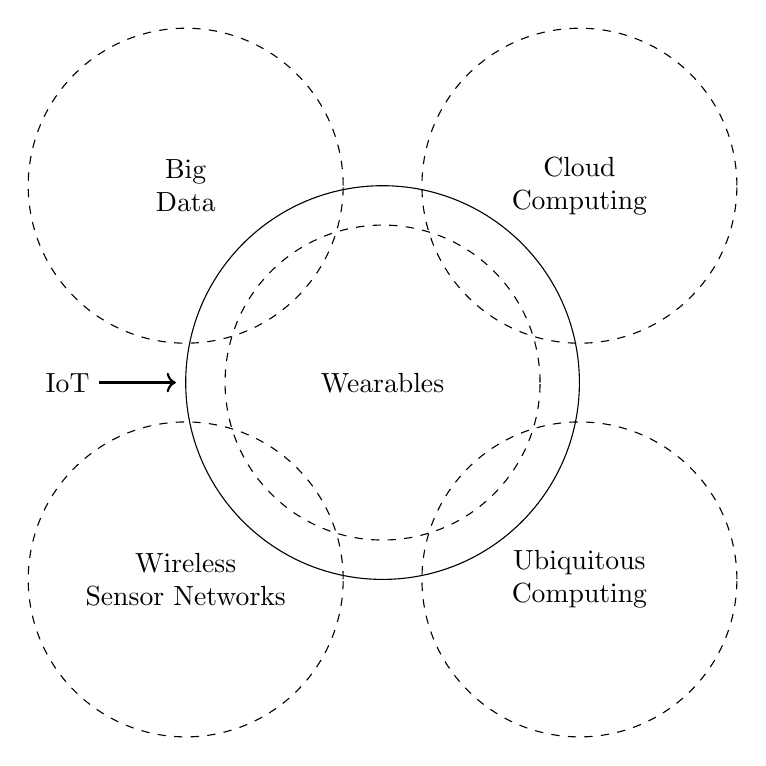
\begin{tikzpicture}
        \node (IoT) at (-2.5,0) {};
        \node at (-4,0) {IoT} edge[->,thick,out=0,in=180] (IoT);
        \draw (0,0) circle [radius=2.5];

        \node[align=center] at (0,0) {Wearables};
        \draw [dashed] (0,0) circle [radius=2];

        \node[align=center] at (-2.5,2.5) {Big\\Data};
        \draw [dashed] (-2.5,2.5) circle [radius=2];

        \node[align=center] at (2.5,2.5) {Cloud\\Computing};
        \draw [dashed] (2.5,2.5) circle [radius=2];

        \node[align=center] at (-2.5,-2.5) {Wireless\\Sensor Networks};
        \draw [dashed] (-2.5,-2.5) circle [radius=2];

        \node[align=center] at (2.5,-2.5) {Ubiquitous\\Computing};
        \draw [dashed] (2.5,-2.5) circle [radius=2];
      \end{tikzpicture}
    \caption{The boundary between IoT and other trends in computing}\label{iotRelationship}
  \end{figure}

  \section{Opportunities}
    Why should we develop IoT solutions? Would our society actually benefit from them? These are the questions posed by stakeholders of all backgrounds. Pilot projects as well as industrial and academic research have shown that there are wide-reaching opportunities to be grasped. Until recently, these opportunities were achievable only in theory or laboratory scenarios, but due to performance improvements and cost reductions in the supporting technology, IoT is very much a reality.

    \citet{fromIoC} describe a number of opportunities created by the evolving technical capabilities of IoT systems. Since much of the value of IoT is derived from the communication of data, the technologies supporting inter-device communication and cooperation are particularly important. Wireless Personal Area Network (WPAN) technologies such as Wi-Fi, Bluetooth, ZigBee and 6LoWPAN give objects the ability to network with Internet resources or each other. These WPAN technologies also provide device addressability mechanisms which allow objects to be uniquely identified from anywhere in the world, through extensions to protocols like MAC Addressing or IPv6. With this level of global interconnectivity, novel services and products become possible.

    Another main characteristic of IoT is the ability to interact with the physical domain. Digital applications will interact with the physical world in two ways: through the monitoring and sensing of physical properties and through the actuation of the physical world in reaction to data. There are a massive variety of sensors available, even to hobby markets, and can measure any imaginable physical property. The reduced cost and improved support by hardware manufacturers will allow measurements to be collected at a scale and precision not previously possible.

    Since IoT microcontrollers are becoming more powerful, there are opportunities for embedded information processing. Embedded information processing refers to end devices performing some form of data processing or storage before transmitting their data; for example, an end device might analyse its own data and only transmit if a specific threshold is met, rather than relying on Cloud Computing-based processing. This is an active area of research called edge computing (or fog computing) and allows for novel methods of data processing and is another method to optimise bandwidth and power consumption.

    Along with these technical capabilities are big-picture societal and economic opportunities. The European Union is a strong example of an economy which can benefit from IoT uptake. The governmental body of the EU, The European Commission, recognises the potential opportunity: ``One major next step in this development [of the Internet] is to progressively evolve from a network of interconnected computers to a network of interconnected objects, from books to cars, from electrical appliances to food, and thus create an ‘Internet of things’.'' In 2009 the Commission published an action plan for embracing the Internet of Things.

    The action plan \citep{ECIoT:2009} describes how IoT will improve citizen well-being both now and into the future. In the present, citizens will benefit from specific IoT initiatives---for instance, Internet-connected health monitoring systems could alleviate pressure on medical services for the ageing society. Other applications such as connected cars or smart waste management are expected to reduce the EU's carbon footprint and therefore protect resources for future generations.

    The Commission's action plan also describes economic opportunties. IoT has the potential to provide many new income streams to businesses as well as finding other money through efficiency savings. First of all IoT opens up new markets which were previously not feasible nor even considered. These markets may include consumer products or novel service solutions in areas such as home security and monitoring. For organisations with complex supply chains or processes, IoT could help to maximise resources and stock control through large-scale automation and efficient information exchange.

  \section{Challenges}
  \label{challenges}
    It is apparent that IoT is still an evolving area of research with numerous challenges to be addressed. In order for IoT to become a mainstream paradigm, the technologies and ecosystem surrounding them must converge and become more mature. \citet{fromIoC} state that IoT is not the result of a single novel technology but rather several complementary technical developments, so invariably, the challenges span many technical disciplines. 

    A good user experience must be offered by these technologies to encourage adoption. \citet{fromIoC} state that devices ``need to establish connections spontaneously, and organize and configure themselves to suit their particular environment'' which they coin `Arrive and Operate'. The process of connecting a laptop to a home Wi-Fi router is representative of the current experience a user might have. They will turn on the Wireless Network Interface Card via a mouse and a Graphical User Interface and select their wireless network before inputing a password with a keyboard. This experience is far from ideal for constrained devices with a simplistic user interface, or no interface at all. The challenge here is to develop technology which allows consumers to use smart objects with little or no configuration.

    Device discovery and interoperability is required to build an open and extensible Internet of Things. Since the world of things is diverse, each type of device is likely to have different capabilities. \citet{interoperability:2015} state that the heterogeneity of existing platforms is considerable (numerous hardware, technologies, requirements and objectives) and as a result, IoT would benefit from a generic architecture which provides IoT developers with a common toolkit. Research efforts have gone some way to address these challenges, such as the IoT `meta-hub' offered by \citeauthor{interoperability:2015}, which provides a feed of available features for a given service.

    IoT infrastructures must be scalable to handle the large number of connections and volume of data. By all estimates, IoT will have a much larger scope and footprint when compared to the existing Internet of computers. The European Commission puts this figure at 50--70 billion devices (on average, 10 per human). \citet{fromIoC} also note that things will be cooperating mainly within a local environment. This means that IoT devices, software and infrastructure must work equally efficiently in both small- and large-scale environments. This complexity is also reflected with the verocity and variety of data being generated; a challenge currently being addressed with research around Big Data.

    Fault tolerance, power supply and efficient wireless communication are challenges facing hardware manufacturers. There are a number of possible operating enviroments for IoT devices, such as office spaces, homes, public spaces and remote areas, so smart objects might depend on a self-sufficient power source. The industry is therefore challenged to produce long-lasting batteries. As well as improving power supply solutions, the industry should maximise power efficiency in other areas such as existing wireless communication technologies which consume too much overhead and power. 

    Technical challenges will continue to be addressed through academic and industrial research, however IoT will not achieve widespread uptake without social acceptance. This is the risk that the industry is carefully attempting to balance; the social acceptance of IoT products is imperative to their success but consumers and markets could be less accepting if industries try too much too soon. The European Commission's action plan describes practical challenges which need to be addressed.

    Many aspects of digital technology is governed by public bodies and the Commission believes that IoT should not be any different. They note that technology will advance due to a normal cycle of innovation and that ``simply leaving the development of IoT to the private section is not a sensible option in view of the deep societal changes that IoT will bring about.'' The main areas which may need to be governed are identification, information security and ethical \& legal accountability. In terms of device identification, \citet{fromIoC} and \citep{ECIoT:2009} suggest that some form public registry (similar to those governed by the Institute of Electrical and Electronics Engineers) will be necessary. In terms of legal accountability, users may be reluctant to use IoT services unless there are safeguards in place. Without effective governance of these areas, IoT may suffer from stifled innovation; a mistrust with data and jeopardised system integrity.

    Standardisation is a technical consideration but also impacts on the economic potential of IoT. The purpose of a standard is to give different entities and stakeholders a common language to design, build or communicate. The widespread adoption of a standard gives businesses of all sizes the opportunity to develop interoperable solutions. In being interoperable, standards-based solutions will be suitable for a wider market and in turn, this will encourage innovation and improve international competitiveness. If IoT is to maximise economic impact and to benefit from widespread adoption, there must be accepted practices or formal standards in place.

    The greatest challenges to social acceptance are security and data privacy, particularly in the EU where the protection of privacy and personal data are two fundamental rights. The challenge with this, in respect to IoT, is that new methods of collecting and using data will be invented. Does current legislation and safeguards protect the interest of EU citizens adequately? Who will own the data---the user whom it is about or the organisation that captured it? The Commission suggests that in response to this challenge, IoT components should be designed from their inception with a privacy- and security-by-design mindset.

  \section{Use Cases}
  \label{use-cases}
    Use-cases are a helpful mechanism for demonstrating the IoT concept. It is a difficult concept to explain because there are many cooperating components and ideas and for this reason, research papers exemplify their arguments with practical examples. Although IoT applications could be developed for virtually any industry there are domains where its application is more obvious. Table \ref{iot-overview} presents six such domains for IoT, together with opportunities, challenges and related areas of research.

    `Smart Cities' is a vision which convincingly demonstrates many benefits of IoT. \citet{DfBIS:2013} describes the main issues facing local authorities which includes: piecemeal urban infrastructure, climate change targets, the changing nature of the high street and elderly social care. The economic downturn has also reduced budgets assigned to local authorities by as much as 30\% between 2010 and 2013 making cost efficiencies another issue. By developing or retrofitting urban infrastructure with IoT connectivity, local authorities can monitor services in much finer detail. For instance, Bigbelly Solar is a smart waste and recycling system. The Internet-connected waste bins allow local authorities to monitor their status and to schedule collections when they are full. \citet{fog:2012} also describe a system of smart, connected traffic lights which can control the traffic flow through a whole city, reducing congestion and improving safety.  

    IoT in the utilities sector is one use-case which has started to become realised. The British Government is requiring energy companies to install smart meters for their customers and expect most to have a smart meter installed by 2020 \citep{DoECC:2013}. Smart meters monitor domestic energy usage on a per-site basis and can give real-time information about how much electricity is being used, expressed in pounds and pence. For individual households this has the benefit of enabling homeowners to save money and to reduce emissions. At a national level, smart meters are a step towards reducing energy consumption and meeting climate change goals. This use case is particularly interesting and well documented, so section \ref{case-study} investigates the smart meter concept further. Additionally, smart thermostats like Nest also allow households to minimise their gas consumption and to reduce heating bills. This is achieved through usage optimisation based on occupancy patterns. 

    Logistics is one area which demonstrates the efficiency savings that an IoT application can make. \citet{ECFreight:2007} states that ``Freight Transport Logistics focuses on the planning, organisation, management, control and execution of freight transport operations in the supply chain'' and notes that it is one of the drivers of European competitiveness. To remain competitive, this industry must continue to improve and streamline infrastructure, fleet management and goods tracking. IoT could be used to share content-related data and location information for regulatory or commercial purposes. This is achieved through the use of inexpensive RFID tags (which store specific information about the item) and GPS sensors (which can identify precise locations). This would reduce time spent by workers manually recording goods and it will reduce errors at interchange points. The Commission has coined this the `Internet for Cargo'.

    \begin{table}
      \scriptsize
      \begin{tabularx}{\textwidth}{|X|X|X|X|X|X|}
        \hline
        \multirow{3}{2cm}{\textbf{Overlapping Research}}
          & \multicolumn{2}{|c|}{\textbf{Opportunities}}
          & \multicolumn{2}{|c|}{\textbf{Challenges}}
          & \multirow{3}{2cm}{\textbf{Example \newline Use Cases}} \\ \cline{2-5}
          & \textbf{Economic \newline \& Societal}
          & \textbf{Technical} & \textbf{Economic \newline \& Societal}
          & \textbf{Technical}
          &
        \\ \hline
          Cloud Computing
          & Citizen Well-Being
          & Communication \& Cooperation
          & Governance
          & `Arrive and Operate'
          & Smart Cities
        \\ \hline
        Big Data
          & Economic Prosperity
          & Addressability
          & Standardisation
          & Interoperability
          & Waste Management
        \\ \hline
          Ubiquitous Computing
          & Ageing Society
          & Identification
          & Security & Discovery
          & Smart Traffic Lights
        \\ \hline
          Wireless Sensor Networks
          & New Markets
          & Sensing
          & Data Privacy
          & Software Complexity
          & Utilities
        \\ \hline
          Wearables
          & Business Optimisation
          & Actuation
          & Trust
          & Scalability
          & Smart Meters
        \\ \hline
          Edge Computing
          &
          & Localisation
          &
          & Data Management
          & Logistics
        \\ \hline
          &
          & Embedded Information Processing
          &
          & Fault Tolerance
          &
        \\ \hline
          &
          & User Interfaces
          &
          & Power Supply
          &
        \\ \hline
          &
          &
          &
          & Wireless Communication
          &
        \\ \hline
      \end{tabularx}

      \caption{A summary of the current state of the Internet of Things}\label{iot-overview}
    \end{table}
    
  \section{Existing Platforms}
  \label{existing-platforms}
    There are a number of IoT platforms both in service and under active development; in fact, Amazon announced their own platform, Amazon IoT, when writing this very comparison \citep{AmazonIoT}. The aim of an IoT platform and the tools which it provides does differ from vendor to vendor, however common characteristics are beginning to emerge. We propose to compare platform offerings across five dimensions: hosting model, source availability model, connectivity, bidirectional communication support and trigger support.

    \subsection{Hosting}
      The hosting model offered by an organisation defines which stakeholder is responsible for maintaining the IoT application and its hardware infrastructure; either the platform provider or the customer. This is a notable differentiator between platforms and can be indicative of the platform vendor's business objectives. There are generally two variations in hosting models: Platform as as Service (PaaS) or self-hosting.

      \subsubsection{Platform as a Service}
        A Platform as a Service (PaaS) is a Cloud Computing concept. It is an abstraction of the complete application technology stack including both hardware and software. An organisation providing a PaaS would be responsible for the management and maintenance of the hardware such as servers, RAID backing storage and networking appliances like routers or switches. Depending on the software on offer, the vendor would also be responsible for managing and maintaining the server operating system as well as any supporting software packages and applications. Customers are typically provided access to this abstraction through a control panel or an Application Program Interface (API).

        \href{https://www.carriots.com/}{Carriots} is an example of a centralised PaaS and their website describes various benefits to a customer \citep{CarriotsBenefits}. Primarily the customer does not need to allocate resources for infrastructure maintenance since this is managed by them, with the result being more time for the customer to focus on business needs. There is also less investment required on behalf of the customer---PaaS resources can be provisioned when and if they are needed, rather than purchasing hardware upfront. Another benefit is the extra layer of support---system scalability, stability and fault tolerance are the responsibility of Carriots.

      \subsubsection{Self-hosted}
        An alternative to a PaaS is the self-hosted option. As the name implies, this option makes customers responsible for the maintenance and management the application infrastructure (although software updates may still be provided by the platform vendor). There are technical and legal arguments to support such a business decision.

        The main technical aspect is that of control. With the self-hosted option, the system architecture can be optimised for specific use-cases, such as the global location of servers to reduce application latencies (the time taken for network transmissions between devices and servers). This also gives customers direct access to the core software and makes it easier to modify it for their own purposes (if the licence or software allows for that).

        Self-hosting may also be necessary for legal compliance, especially in the realm of data protection. Depending on the country of operation, it may be necessary to retain data within country boundaries and this may not be enforceable with a PaaS. In October 2015 the Court of Justice of the European Union ruled that the Safe Harbour agreement between the EU and United States is invalid \citep{C362/14}. This case found that the United State's data protection legislation was not adequate and means that any organisation sharing data under this agreement is now acting unlawfully. This problem could be avoided, or at least remedied more quickly, if data is managed from within the European Union. One example of a self-hosted platform is \href{http://nitrogen.io/}{Nitrogen.io}.

        % TODO: Expand on Nitrogen.io

    \subsection{Source Availability Model}
      The Source Availability Model chosen by a platform developer defines the level of accessibility for their source code. This model comes in two forms---open or closed source---and can be further refined by a software license framework.

      The source code of Open Source Software (OSS) is made publicly available. This could be served as a standard file download or, as is becoming common practice, on a code sharing service such as Github or Bitbucket. OSS will typically be provided under the conditions defined in a license, such as the GPL, MIT or Apache license frameworks. These vary on points like distribution, modification and notification of copyright \citep{license:2015}.

      Closed Source Software is proprietary source code not made publicly available, although it may be necessary to distribute compiled binaries. This just means that the organisation does not wish to make source code available for modification or knowledge sharing. 

      In conjunction with the hosting model, the source availability is indicative of business objectives. Organisations wishing to commercialise their platform as a product offering will use a Closed Source model to protect their intellectual property. Conversely those organisations where knowledge sharing is an aim, or where the platform is a mechanism to sell other products or services (such as \href{https://data.sparkfun.com/}{Sparkfun} and their electronic hardware) may use an Open Source model.

    \subsection{Connectivity}
      The IoT concept \emph{is} interconnectivity and communication, making device and application connectivity a very important topic. The platforms investigated support a range of connectivity protocols and concepts. These range from widely-accepted HTTP-based APIs to more niche protocols like CoAP and MQTT.

      \subsubsection{HTTP}
        The Hypertext Transfer Protocol (HTTP) underpins the internet. It benefits from widespread support and most notably, is used by web browsers to interface with web servers. RFC 2616 \citep{rfc2616} defines the specification for HTTP version 1.1 and notes:

          \begin{quote}It is a generic, stateless, protocol which can be used for many tasks beyond its use for hypertext, such as name servers and distributed object management systems, through the extension of its request methods, error codes and headers.\end{quote}

        As hinted at by this RFC 2616 quote, three important features of HTTP are: request methods, error codes and headers. To generalise the HTTP lifecycle, a user agent will send a request to an origin server, the server will process the request and will return a response. The request will use an HTTP \emph{verb} to define the action to take, such as \code{GET} or \code{POST}, and will include headers to specify other parameters. The response has an associated status code, such as \code{200 OK} or \code{404 Not Found}.

        Most of the platforms investigated here support HTTP requests through a Representational State Transfer (REST) API. \citet{rest:2000} states that the REST architectural style emphasises scalability, independence of components, minimises latency and maximises security. These characteristics are achieved by applying constraints to the application, such as stateless communication, a uniform component interface and a layered approach to infrastructure technologies. REST methods are based on the HTTP verbs like \code{GET}, \code{POST}, \code{PUT} and \code{DELETE}. For IoT application developers, a REST API provides a scalable, uniform and robust interface between devices and the Internet.

        Software engineers working on specifications for the Internet have foreseen the Internet of Things, even if it was taken in jest. RFC 2324 \citep{rfc2324} is an April Fool's joke and defines the Hyper Text Coffee Pot Control Protocol version 1.0 (HTCPCP/1.0). It specifies methods by which an Internet-connected coffee pot can be controlled, and even adds a new error code: ``Any attempt to brew coffee with a teapot should result in the error code `\code{418 I'm a teapot}'. The resulting entity body MAY be short and stout.''

      \subsubsection{WebSockets}
        The WebSocket Protocol is an independent TCP-based protocol that enables two-way communication. It uses an HTTP request as part of the handshaking process, which is treated as a connection upgrade request. RFC 6455 \citep{rfc6455} states ``The goal of this technology is to provide a mechanism for browser-based applications that need two-way communication with servers that does not rely on opening multiple HTTP connections (e.g., using \code{XMLHttpRequest} or \code{\textless iframe\textgreater}s and long polling).'' This technology plays a vital role in enabling bidirectional communication between web browsers and servers, as will be covered in section \ref{bidirectioncomms}.

        WebSockets use standard HTTP ports for communication by default (port 80 and 443 for unencrypted and encrypted connections respectively). This has the added benefit of being compatible with common network and firewall configurations.

      \subsubsection{MQTT}
        MQ Telemetry Transport (MQTT) is a simple and lightweight messaging protocol. It is based on a publish/subscribe model and is specifically designed for constrained devices and low-bandwidth, high-latency or unreliable networks. In general, MQTT is used in conjunction with a message broker. Clients subscribe to topics on this broker which will then forward any relevant messages. Clients are then free to do whatever they please with these messages \citep{mqtt:2015}.

        MQTT uses TCP/IP to transmit messages and operates on ports 1883 and 8883 for unsecured and secured uses respectively. Since these ports and not common, firewalls will typically block access. For this reason, MQTT can be tunnelled using WebSockets (and means this can be used in the browser, too).

      \subsubsection{CoAP}
        Constrained Application Protocol (CoAP) is another protocol designed with the Internet of Things in mind. \citet{rfc7252} describe CoAP as ``a specialised web transfer protocol for use with constrained nodes and constrained networks.'' Some headline features align with principles used with HTTP, such as utilisation of the REST model. RFC 7252 defines the proposed specification for CoAP. It specifically notes some main features:

        \begin{itemize}
          \item Web protocol fulfilling M2M requirements in constrained environments
          \item UDP [RFC0768] binding with optional reliability supporting unicast and multicast requests
          \item Asynchronous message exchanges
          \item Low header overhead and parsing complexity
          \item URI and Content-type support
          \item Simple proxy and caching capabilities
        \end{itemize}

        CoAP is likened to HTTP throughout the specification however there are some notable differences. HTTP uses the TCP/IP transport protocol whereas CoAP uses UDP, a protocol with significantly less overhead. UDP is not a request/response protocol so to provide a request/response interaction model, CoAP must deal with this through a logic layer.

      \subsubsection{UDP}
        One of the researched platforms also offers the User Datagram Protocol (UDP) as a connectivity option. RFC 768 \citep{rfc768} notes ``this protocol provides a procedure for application programs to send messages to other programs with a minimum of protocol mechanism.'' To achieve `a minimum of protocol mechanism', UDP does not establish a connection with the receiving device, so unlike TCP/IP it is connectionless. The protocol also specifies no mechanism for error correction so if a packet is lost in transit, it is lost forever.

        Since data can be lost, this protocol should only be used in applications which can tolerate data loss. To give a real-world example, a battery-powered hygrometer sensor may be collecting data about the enviromental humidity. If UDP was used as the connectivity protocol, it would allow this sensor to wake up, transmit its reading and then fall back to sleep without being concerned about the packet's progress. If a packet was lost, it would not have business or safety impacts.

    \subsection{Bidirectional Communication}
    \label{bidirectioncomms}
      One main opportunity of IoT, as described in Section \ref{TechnicalOpportunities}, is to drive actuators in response to data. There are three aspects which define whether unidirectional or bidirectional communication is possible: the connectivity protocol, the software application and the network environment. To illustrate the following points, a hypothetical scenario will be used, where one server and one actuator are connected together through the internet. In this case, unidirection communication means that only the actuator can initiate network requests whereas bidirectional communication allows either the server or actuator to initiate.

      If the actuator is publicly addressable with a dedicated IP address, bidirectional communication is trivial to implement. Supposing that the HTTP protocol is being used for communication, both the actuator and server can initiate requests to each other by using the appropriate IP address. The server may send an HTTP request instructing the actuator to do something. In real-world scenarios, there are three factors which make bidirectional communication like this difficult: firewalls, Network Address Translation and IPv6 uptake.

      Firewalls are common-place both in businesses and at home. They are a network security tool and can be either a dedicated hardware unit or software built into other devices, such as a domestic router. Their purpose is to screen both in and outbound connections which may have a malicious or compromising effect on the network integrity. The side effect which this has on IoT systems is that non-common protocols may be blocked, such as MQTT (since it uses ports 1883 and 8883). While devices behind a firewall may be publicly addressable, they may not be reachable, depending on the IoT application.

      While obtaining a public IP address for each IoT device is a worthy aim, it is not achievable in many situations due to Network Address Translation. Network Address Translation (NAT) is a tool used to delay the depletion of IPv4 addresses and is very common with domestic internet connections. RFC 2663 \citep{rfc2663} states ``NAT devices are used to connect an isolated address realm with private unregistered addresses to an external realm with globally unique registered addresses.'' In essence, this allows a number of privately addressed devices to communicate through one public address. In terms of IoT, this means than any devices connected behind NAT will not be publicly addressable---the server can not directly send a request to the actuator.

      Internet Protocol version 6 (IPv6) will solve the issue of IP address depletion. It will offer over 340 undecillion possible addresses, compared to just under 4 billion available from IPv4, and will allow every connected device to have its own IP address for the foreseeable future \citep{ipv6:2008}. With regards to the Internet of Things, this is still not achievable. IPv6 is still not supported by many internet service providers (ISPs) and networks, including that of Robert Gordon University. For the Internet of Things, this means that universally supported IPv6 is still a while off.

      There are some useable techniques to overcome these three issues and to enable (or mimic) bidirectional communication. The first of these solutions is HTTP polling. With standard polling, the actuator would periodically ask the server for updates. If this period was 1 second, the communication may feel like it was real-time and bidirectional. This is however wasteful because not every request will result in an update. A more efficient form of polling is called long polling. The actuator will send a request to the server, but if there are no updates yet, the server will not respond. When the server does have a message to send to the actuator, it will respond and then end the request. This is better, but implementations suffer from the added complexity of managing connections.

      A final and more effective solution is to implement communication using WebSockets. As previously described, the WebSocket protocol allows for bidirectional, full duplex communication and it can solve every challenge already addressed. WebSockets use the same communication ports as HTTP (port 80 and 443) by default, meaning that firewalls will allow them. Networks that support web browsing will support WebSockets. Also, the WebSocket connection can be initiated by the client and still allow bidirectional communication. In this case, the actuator can open a WebSocket connection to the server and overcome any Network Address Translation in place because it does not require a public IP address.

    \subsection{Application Triggers}
      An application-level feature common across investigated platforms is event triggers or rules. Where supported, platforms can trigger actions based on the data received from sensors and third-party APIs. Combining examples already mentioned, a hygrometer may send data to an IoT application. An application trigger could be configured to turn on a dehumidifier actuator if the humidity passes a certain threshold. If bidirectional communication is supported, this trigger would react in real-time. Triggers could also be configured to interact with other third-party software APIs.

      \begin{table}
        \scriptsize
        \begin{tabularx}{\textwidth}{|X|X|X|X|X|X|}
          \hline
          \textbf{Service} & \textbf{Hosting} & \textbf{Source} & \textbf{Connectivity} & \textbf{Bidirectional} & \textbf{Triggers} \\ \hline
          Amazon IoT & PaaS & Closed & MQTT, HTTP & Yes & Yes \\ \hline
          Bug Labs Dweet & PaaS & Closed & HTTP & Yes (app) & No \\ \hline
          Carriots & PaaS & Closed & HTTP, MQTT & No & Yes \\ \hline
          Sparkfun & PaaS or self-hosted & Open & HTTP & No & No \\ \hline
          Exosite & PaaS & Closed & CoAP, HTTP, UDP & No & Yes \\ \hline
          Google Brillo & PaaS & Closed & Unknown & Unknown & Unknown \\ \hline
          Digi & PaaS & Closed & HTTP & Yes & Yes \\ \hline
          IFTTT & PaaS & Closed & HTTP & No & Yes \\ \hline
          Newaer & PaaS & Closed & HTTP & No & Yes \\ \hline
          Nimbits & Self-hosted & Open & HTTP & No & Yes \\ \hline
          nitrogen.io & Self-hosted & Open & MQTT, HTTP & Yes & Yes \\ \hline
          ThingSpeak & PaaS or self-hosted & Open & HTTP & No & Yes \\ \hline
        \end{tabularx}

        \caption{Characteristics of existing IoT platforms}\label{platform-characteristics}
      \end{table}
  \section{Sensor Hardware}
  \label{sensor-hardware}
    The Internet of Things is a multidisciplinary area of research and is just as dependant on advancements in electrical and electronics engineering as it is computer science. Since the hardware driving IoT sensor nodes is intertwined with the upper layers of software, it would be appropriate to investigate the current state of this area too. Rather than research the intricacies of how these pieces of hardware work, this paper will investigate existing end device hardware with regards to their implementation in IoT applications, particularly technical capability and energy efficiency.

    With a similar method to Section \ref{existing-platforms}, various makes and models of hardware boards were analysed to find comparable characteristics. The manufacturers chosen---Arduino, Raspberry Pi, Intel and Samsung---represent a cross-section of the field. These manufacturers aim their products at different markets, from the DIY `maker' market of the Arduino to the professional, consumer electronics market of Samsung. This section will compare and contrast hardware models produced by these manufacturers across a range of key areas: processor architecture, memory, input/output options and wireless connectivity. Table \ref{hardware-boards} summarises each model and their specifications.

    \subsection{Processor Architecture}
      Just like any other computer system, the processor is the heart of the hardware board. It is responsible for running the operating system, orchestrating the various system components and for running the user application. The type and specification of the processor defines what can be processed and how quickly, which is ultimately reflected in the responsiveness and capability of the IoT device. Processor throughput is not the only consideration when scoping an IoT device however---energy consumption is also an important factor. The specification of the processor can be categorised into smaller areas: processor type, instruction set, number of bits, clock speed and the number of cores.

      There are two broad types of processor systems, namely microcontrollers and microprocessors. A microcontroller (also known as an embedded controller) is a complete computer in one chip. A single microcontroller chip will typically combine a central processing unit (CPU), small amounts of program memory and Random Access Memory (RAM) and input/output lines \citep{microcontrollers:2011}. In comparison, a microprocessor requires other system components to function, such as external memory, input/output lines and a clock circuit. In this regard, microprocessor hardware cannot be upgraded because it is integrated whereas a microprocessor system can, but they are cheaper to manufacture.

      Processor architecture can also vary between makes and models. \citep{microcontrollers:2011} notes that processors can be classified by the number of bits they process, with 8 bits being the most popular for microcontrollers. Processors with a greater number of bits are more powerful but are also more expensive. The instruction set used also effects the performance of the processor; Reduced Instruction Set Computer (RISC) instructions take only one CPU cycle to complete whereas Complex Instruction Set Computer (CISC) instructions can take multiple cycles.

      Clock speed and the number of cores are two final factors of a processor's performance. The clock speed describes how many cycles the CPU executes in one second and is regulated by a crystal timer or internal digital clock oscillator (DCO) A greater clock frequency means more instructions which can be processed in a time period, and the more powerful the processor. Microcontrollers typically have clock speeds in the tens of Megahertz whereas microprocessors might run at hundreds of Megahertz or a number of Gigahertz. However due to physical limitations of hardware components, there is a practical limit in possible clock speed. In this case more cores are added to the processor allowing it to evaluate multiple instructions concurrently. With regard to power consumption, \citet{wsnpower:2010} state that clock speed is one factor affecting the lifetime of a battery powered device so the CPU should be carefully considered for its application.

    \subsection{Memory}
      In any computer system, different types of memory are used to store program instructions and the temporary data associated with them. While these types of memory can be split into more discrete categories, there are generally two types of memory: non-volatile and volatile. Non-volatile memory, such as Read-Only Memory (ROM) or Programmable Read-Only Memory (PROM), is used to store program instructions and fixed user data. Non-volatile memory is used to store this kind of data because it is not lost when power is disconnected. In comparison, volatile memory loses its contents when power is removed and so it is used for temporary or intermediate data.

      Memory characteristics also contribute to the capabilities and performance of the hardware system. Primarily, the available memory size defines how much data can be stored. The Arduino boards researched have 32KB of program memory available compared to the Gigabytes available on some Samsung Artik boards. This constrains the number of program instructions which can be stored and means the software running on the Samsung Artiks could be much more complex. Memory word length also has implications. The word length is the number of bits which a single unit in memory can store, and is commonly found to be 8, 16, 32 or 64 bits. Larger word lengths can store larger pieces of instructions or data, such as larger numbers. 

    \subsection{Input/Output}
      The Input/Output (I/O) lines of a hardware board are the interface between sensors or actuators and the processor (or beyond). Without this physical connectivity, developers would not be able to capture information about the physical world, stopping the IoT concept in its tracks. This aspect of hardware boards is therefore important to the flexibility and future potential of IoT applications. To ensure compatibility between hardware platforms and external hardware like sensors, various industry standards have been developed.

      Before any I/O standards are discussed though, it is first important to establish the importance of the operating voltage for an individual electronics circuit. The hardware boards analysed operate at various logic voltages; for instance most Arduino boards run at 5V whereas the native voltage of the Intel Edison is 1.8V. The standard logic voltage also effects I/O operation. Digital sensors may have their own, incompatible standard logic voltage---a microcontroller running at 5V would damage a sensor running at 3.3V. If directly interfacing between processors and sensors, a logic level shifter might have to be implemented so careful planning is required. Logic voltage is another aspect which affects the lifetime of a battery-powered node \citep{wsnpower:2010}.

      General Purpose Input Output (GPIO) pins are a blank canvas for engineers and developers. They are digital I/O pins with no default use and as their name suggests, can be configured as input or output. Since they are digital, GPIO pins can only read or write with 2 discrete values, logic high (1) or logic low (0), and these values usually respect the standard system voltage. Depending on the device, a number of GPIO pins might support Pulse Width Modulation (PWM). PWM is a technique for emulating analogue levels by pulsing the digital value at differing frequencies. Using a light bulb as an example, PWM could emulate the effect of dimming the light, like what could be achieved with an analogue potentiometer.

      While GPIO pins allow for basic I/O operations, there is a need for communicating with more complex data. There are various available standards for interfacing between low-level electronics components. The datasheets for the selected model note some common standards, namely: Serial Peripheral Interface (SPI), Universal Asynchronous Receiver/Transmitter (UART), Inter-Integrated Circuit (I\textsuperscript{2}C) and Integrated Interchip Sound (I\textsuperscript{2}S). There are a variety of uses for these standards so this paper will go no further than noting that they exist.

    \subsection{Connectivity}
      Interconnectivity is yet one more important aspect to hardware designed for the Internet of Things. Since IoT devices are becoming increasing mobile and wire-free, connectivity is being discussed almost exclusively in regards to wireless communication protocols and standards. As was discussed in Section \ref{TechnicalOpportunities}, some IoT-specific wireless standards have already been established. Many of these technologies are supported by the various hardware platforms investigated, validating their purpose. The standards supported by these hardware platforms are IEEE 802.11 (Wi-Fi), Bluetooth and IEEE 802.15.4 (Low-Rate Wireless Personal Area Network). 

      Wi-Fi is a technology which has become synonymous with wireless connectivity and the Internet. The IEEE 802.11 standard states that the purpose of Wi-Fi is ``to provide wireless connectivity for fixed, portable, and moving stations within a local area'' where a local area could refer to a home, classroom or office space. Wi-Fi benefits from wide utilisation in all areas and industries so wireless coverage is likely to be in place already. \citet{wifiah:2012} state that the radio frequencies used by Wi-Fi (2.4GHz and 5GHz bands) are becoming crowded and are increasingly resulting in radio interference. This is being addressed in a new standard, IEEE 802.11.ah, which makes use of the 900MHz frequency band. The two main potential advantages of this standard are greater range and less power consumption, which is beneficial to IoT devices. Even with this standard, however, end devices are impeded by the large overhead of upper layer protocols used in conjunction with Wi-Fi.

      The Bluetooth standard has been repurposed as an effective wireless communication protocol for IoT devices. Prior to the introduction of Bluetooth 4.0 in 2010, it was primarily used in multimedia applications such as streaming stereo audio \citep{bluetooth:2014}. With the introduction of Bluetooth 4.0 came new features, namely Bluetooth Low Energy (BLE), which consumes such a small amount of power that a sensor can run from a coin battery for months or years. For an average usage scenario, BLE could be expected to achieve a practical maximum range of 77 meters \citep{linklabs:2015} which makes it ideal for use-cases such as body sensors and intelligent transport systems.

      One final wireless connectivity standard supported by the investigated hardware is IEEE 802.15.4 Low-Rate Wireless Personal Area Networks (WPAN). The standard states that it `` provides for ultra low complexity, ultra low cost, ultra low power consumption, and low data rate wireless connectivity among inexpensive devices'' and covers the physical layer (PHY) and Medium Access Control (MAC) sublayer specifications. This IEEE standard has manifested into various competing technologies, in particular ZigBee and 6LoWPAN. ZigBee is a set of layers built on top of 802.15.4 and adds three important features: routing, ad-hoc network creation and self-healing mesh \citep{buildingWSN:2010}. In comparison, 6LoWPAN is an adaptive layer defined in RFC 4944 and allows IPv6 packets to be transmitted using the short addresses in 802.15.4 \citep{IPisDead:2008}. The average range for ZigBee and 6LoWPAN is 291 and 191 meters respectively \citep{linklabs:2015}.

      \begin{sidewaystable}
        \centering
        \scriptsize
        {\setlength{\extrarowheight}{5pt}%
        \begin{tabular}{|l|l|c|c|c|c|c|c|c|c|c|l|}
          \hline
            \multicolumn{2}{|c|}{\textbf{Board}}
            & \multicolumn{3}{|c|}{\textbf{Processor}}
            & \multicolumn{2}{|c|}{\textbf{Memory}}
            & \multicolumn{3}{|c|}{\textbf{Input/Output}}
            & \multirow{2}{*}{\textbf{Voltage}}
            & \multirow{2}{*}{\textbf{Connectivity}}
          \\[5pt] \cline{1-10}
            \textbf{Make}
            & \textbf{Model}
            & \textbf{Bits}
            & \textbf{Cores}
            & \textbf{Speed}
            & \textbf{App}
            & \textbf{RAM}
            & \textbf{Analogue}
            & \textbf{Digital}
            & \textbf{PWM}
            &
            &
          \\[5pt] \hline
            \multirow{3}{*}{Arduino}
            & Uno
            & 8
            & 1
            & 16MHz
            & 32KB
            & 2KB
            & 6
            & 14
            & 6
            & 5V
            & -
          \\[5pt] \cline{2-12}
            & Yún
            & 8
            & 1
            & 16MHz
            & 32KB
            & 2.5KB
            & 12
            & 20
            & 7
            & 5V
            & \parbox[t][0.7cm][t]{2cm}{Ethernet \newline Wi-Fi}
          \\[5pt] \cline{2-12}
            & Pro Mini
            & 8
            & 1
            & 8MHz/16MHz
            & 32KB
            & 2KB
            & 6
            & 14
            & 6
            & 3.3V/5V
            & -
          \\[5pt] \hline
            \multirow{3}{*}{\parbox[t]{1.3cm}{Raspberry \newline Pi}}
            & 2
            & 32
            & 4
            & 900MHz
            & SD Card
            & 1GB
            & 0
            & 40
            & 0
            & 5V
            & Ethernet
          \\[5pt] \cline{2-12}
            & A+
            & 32
            & 1
            & 700MHz
            & SD Card
            & 256MB
            & 0
            & 40
            & 0
            & 5V
            & -
          \\[5pt] \cline{2-12}
            & Zero
            & 32
            & 1
            & 1GHz
            & SD Card
            & 512MB
            & 0
            & 40
            & 0
            & 5V
            & -
          \\[5pt] \hline
            Intel
            & Edison
            & 64
            & 2
            & 500MHz
            & 4GB
            & 1GB
            & 6
            & 20
            & 4
            & 1.8V/3.3V
            & \parbox[t][0.7cm][t]{2cm}{Wi-Fi a/b/g/n \newline Bluetooth 4.0}
          \\[5pt] \hline
            \multirow{3}{*}{Samsung}
            & Artik 1
            & 32
            & 1
            & 240MHz
            & 4MB
            & 1MB
            & 2
            & 0
            & 0
            & Unknown
            & Bluetooth 4.0
          \\[5pt] \cline{2-12}
            & Artik 5
            & 32
            & 2
            & 1GHz
            & 4GB
            & 512MB
            & 2
            & 47
            & 2
            & 1.8V/2.4V
            & \parbox[t][1cm][t]{2cm}{Wi-Fi a/b/g/n \newline Bluetooth 4.0 \newline ZigBee/802.15.4}
          \\[5pt] \cline{2-12}
            & Artik 10
            & 32
            & 4+4
            & 1.3GHz/1GHz
            & 16GB
            & 2GB
            & 6
            & 51
            & 2
            & 1.8V/2.4V
            & \parbox[t][1cm][t]{2cm}{Wi-Fi a/b/g/n \newline Bluetooth 4.0 \newline ZigBee/802.15.4}
          \\[5pt] \hline
        \end{tabular}}

        \caption{Summary of hardware boards}\label{hardware-boards}
      \end{sidewaystable}

  \section{Case Study: UK Smart Meters}
  \label{case-study}
    \subsection{Overview}
      The smart meter project by the British government serves as an ideal case study to exemplify an Internet of Things application. In Section \ref{use-cases}, this paper described some stand-out use cases, which were collated from various sources. Upon researching the smart meter concept further, this massive governmental project---currently being developed for the United Kingdom utilities sector---was discovered. As more research on this project was carried out, it became clear that it represents a significant commentary in regard to the IoT concept.

      In comparison to other potential case studies, the smart meter project is important for many reasons. First of all, the transparent and objective nature of public projects does prevent an operational bias. It would be possible to evaluate case studies provided by commercial organisations; for instance, Digi provide case studies across a number of industries. This however introduces the risk of bias---it is in the business's interest to make a sale. In order to satisfy stakeholders, it is also necessary for the public project to unambiguously document discussions, actions and expectations. Furthermore, the scale, purpose and complexity of this project truly puts the Internet of Things concept to the test.

      Before analysing the technical details of this project, it is first important to understand the purpose of smart meters. The project was announced by the Department of Energy and Climate Change (Decc) in 2009. It ambitiously aims to replace the electricity and gas meters for all residents of the United Kingdom with so-called `Smart Meters' by 2020, giving a projected time frame of 10 years \citep{SMannouncement:2009}. For consumers, these systems comprise of two main components: the electricity/gas meter and the in-home display. The display will wirelessly connect to the meter and will provide a near real-time indication for the resources being consumed, expressed in pounds and pence \citep{SMguide:2013}. Utility companies will also be provided with remote access to the meter, primarily allowing them take readings.

      With an estimated cost of £10.9 billion \citep{SMthirdreport:2014}, the project must deliver benefits to consumers, suppliers and the government. One of the main drivers for meters are the potential financial savings. For the consumer, they are more aware of their own energy usage which allows them to reduce their spending. Into the future, this could become automated with Smart Appliances which wait for cheap energy. For the supplier, large savings will be made through the automation of meter readings and billing. Operational maintenance will also become streamlined as smart meters can immediately identify faults. For the government, efficiency savings will reduce the national environmental impact and will help the United Kingdom meet climate change targets \citep{SMUK:2012}. The total projected savings from the combination of these points is £17.1 billion, resulting in a net benefit to the British economy of at least £6 billion \citep{SMthirdreport:2014}.

    \subsection{Governance}
      Effective governance and organisation is imperative for the success of the smart meter roll-out in the United Kingdom. Governance was discussed, in board terms, as part of Section \ref{economic-societal-challenges} and found three main areas which may require governing: device addressability, information security and ethical \& legal accountability. Similar issues face the British government. The Department for Energy and Climate Change have been responsible for managing the smart meter programme since April 2012 and delegates governing roles to various actors in the project. Some of the main actors include the Office of Gas and Electricity Markets (Ofgem), the purpose-built Data and Communications Company (DCC) as well as various subcontractors and licensees. These bodies govern the smart meter project roll-out across many areas, including two which are of special interest to this paper: consumer protection and technical implementation.

      Widespread social acceptance is one of the main challenges facing IoT products and services; consumer protection offered by Decc and its subcontractors goes some way to earn this public trust. First and foremost, the energy data generated by smart meters is useful to consumers, suppliers and the government. In response to the privacy issues which this creates, the Decc has developed the Data Access and Privacy Framework (DAPF). \citet{DataAccess:2015} notes that this governing framework serves three main purposes:

      \begin{itemize}
        \item{Protect consumers’ interests, including by addressing concerns that consumers may have about privacy;}
        \item{Enable proportionate access to data by authorised parties to ensure that benefits can be delivered; and}
        \item{Promote competition and innovation in the developing energy services market.}
      \end{itemize}

      The DAPF is expected to be finalised by 2018. The Decc also addresses specific consumer concerns with governance and legislation. For instance, there are restrictions in regards to the supplier-led installation as detailed by the Smart Meter Installation Code of Practice, including: prohibition of sales during installation visits and the mandatory provision of energy advice.

      Governance also extends to the technical standards and specifications used for the smart meter project. One important challenge facing this project is hardware and software interoperability between the large number of parties. The Smart Metering Equipment Technical Specifications (SMETS) document was drawn up in 2012 and represents the technical standards to be followed by suppliers and systems developers for the in-home products. The responsibility of Wide Area Network communication has been delegated to the Data and Communications Company (DCC). This organisation specifies its own standards for connecting to the WAN, which go as far as XML schema for inter-system communication.

    \subsection{Implementation}
      From the perspective of this paper, the technical implementation is the most interesting aspect of the smart meter project. There is a huge level of complexity and interconnectivity covered by SMETS and DCC specifications. The completed system will be a distributed and connected platform for smart meters in the United Kingdom and can be split into three constituent components: energy consumers, wide-area connectivity and service users. The implementation is summarised in Figure x.x.

      Before discussing the implementation of specific technologies it is first worthwhile to understand the high-level system architecture. The energy consumers for the smart meter project are homes and small businesses. As was previously noted, there are three product types which each premises will have: smart meters (gas and electric), in-house displays and communication hubs. The communication hubs have two responsibilities, namely to provide premises-wide wireless connectivity---dubbed the Smart Meter Home Area Network (SM HAN)--- and to connect each SM HAN to the nationwide Wide Area Network (WAN) provided by the Data and Communications Company. Service users are the utility companies like British Gas or Scottish and Southern Energy (SSE) as well as authorised third-parties such as online energy comparison websites. Authorised service users will gain bidirectional connectivity with their customer's smart meters through the DCC WAN.

      The SMETS and Communications Hub Technical Specification (CHTS) documents complement one another to unambiguously define the functional requirements for smart meters and the home area networks. Since the communication hub will provide wireless connectivity across a single premises, its functional requirements are indicative of how this network will operate. \citet{chts:2014} state that the HAN interface of the communications hub will use ZigBee over the 2.4GHz frequency band. The CHTS also notes the minimum capacity of the SM HAN: four Electricity Smart Metering Equipment (ESME), one Gas Smart metering Equipment (GSME), one Gas Proxy Function (GPF), seven Type 1 devices and three Type 2 devices. Type 1 devices are those which can issue any command to ESME or GSME meters whereas Type 2 devices can only issue read requests \citep{EnergyUtilities:2014}.

      Individual metering devices have their own functional requirements which will inform their hardware implementation. The high-level expectations of a ESME or GSME device are: a clock, a data store, meter containing one measure element, a HAN interface, a load switch, a Random Number Generator and a user interface \citep{smets:2014}. It is also important to note that ESME or GSME devices must be capable of storing 13 months of readings taken at 30-minute intervals, even after power loss. \citet{SMUK:2012} compared the UK requirements against an existing smart meter, the Elster REX2. This meter has has an 8-bit Texas Instrument SoC with a clock speed of 32MHz, 4KB of RAM, 256KB of application memory along with 21 GPIO lines and up to 8 analogue inputs. These specifications would place the required hardware in the realm of the Arduinos researched in \ref{sensor-hardware} however the authors argue that the UK devices would need to be more powerful and with greater memory due to the data storage and potential computational requirements.

      The final piece to the smart meter project is the Wide Area Network managed by the Data and Communications Company. The DCC is responsible for secure communication, access control and scheduled data retrieval for this project. Since the installation environments will differ from premises to premises, various connectivity methods are being employed, such as cellular, broadband and 802.15.4 mesh radio. This is, in essence, the platform supporting the whole project. The DCC will maintain a web-based service where service users can issue HTTP requests with XML document payloads to achieve tasks. The possible functions are defined in the DCC User Interface Specifications (DUIS).

  \section{Conclusions}
    \chapter{Specification}
\label{Chapter:Specification}
  To obtain a complete and practical understanding of the IoT paradigm, the software implementation accompanying this paper will comprise of two distinct components: a generic IoT application framework and a demonstration application. \citet{interoperability:2015} state that developers of IoT applications would benefit from a generic, standardised architecture, and that is the aim of the framework component. The second component has two main purposes. First of all, it will implemented the framework component with the aim of validating design decisions. The second purpose is to demonstrate the opportunities present in IoT. This chapter will define the requirements for both of these components.

  To help reference these two software components throughout the remainder of this paper, they have been given product names. Haar is a cold sea fog which forms on the east coast of Scotland and is a fitting metaphor for IoT being all around us. It is also a nod towards the Fog Computing paradigm, and towards Robert Gordon University's location in Aberdeen. The generic framework will be called Haar Engine and the demonstration application will be named Haar.

  \section{Functional Requirements}
    \subsection{Framework}
      The target users of Haar Engine are designers and developers of IoT services and applications. The general aim of a framework is to encapsulate design decisions into a logical and elegant toolkit. Haar Engine aims to perform the same task by encapsulating the knowledge which has been collated in Chapter \ref{Chapter:Background}. The following subsection specifies its main requirements.

      \subsubsection{User and Device Management}
        The following requirements have been derived from the analysis of existing platforms and the requirements of use cases.

        \begin{enumerate}
          \item The framework shall model users
          \begin{enumerate}
            \item A user shall be identified by a unique username
            \item A user shall have an associated profile including: full name, email address
            \item Users shall be assigned a privilege level: standard or administrator
          \end{enumerate}
          \item The framework shall authenticate genuine users only

          \item The framework shall model connected IoT devices
          \begin{enumerate}
            \item A device shall be identified by a unique identification number
            \item A device shall be designated as either an input (sensor) or output (actuator)
          \end{enumerate}
          \item The framework shall authenticate genuine devices only

          \item The framework shall authorise and facilitate the management of devices
          \begin{enumerate}
            \item A device will have one owner
            \item Access to device data and configuration options shall be restricted to the device owner by default
            \item The device owner shall be able to make device data public
            \item A device owner shall be able to grant access permission to specified users
          \end{enumerate}
        \end{enumerate}

      \subsubsection{Device Connectivity}
        Haar Engine is responsible for managing the connectivity between devices and itself. The issues surrounding bidirectional communication was described in Section \ref{bidirectioncomms}, and these should be addressed by this framework.

        \begin{enumerate}
          \item The framework shall establish a connection with end devices
          \begin{enumerate}
            \item Devices shall be addressable and identifiable whilst the connection is open
            \item The connection shall remain open under normal operating conditions
            \item Under error conditions, the connection shall be re-established
          \end{enumerate}
          \item The connection shall be bidirectional
          \begin{enumerate}
            \item Input devices shall be able to transmit data packets to the framework
            \item The framework shall be able to transmit data packets to output devices
            \item The connection shall be tolerant of network obstacles such as firewalls and Network Address Translation
          \end{enumerate}
        \end{enumerate}

      \subsubsection{Data Storage}
        IoT applications will collect a large volume of data. The data collected by these applications will vary in structure and type, so Haar Engine must be tolerant of this. The developers potentially using this framework will have specific domain knowledge and so should be empowered to tailor the system for their needs.

        \begin{enumerate}
          \item The framework shall store data received by devices
          \item The framework shall provide an interface for using different database types
          \begin{enumerate}
            \item The framework shall provide a default `out of the box' database connector
            \item Application developers shall be able to create their own database connectors
          \end{enumerate}
        \end{enumerate}

      \subsubsection{Data Access API}
        Haar Engine must be able to provide access to stored data. Primarily this access will be for use in its own application, however third-party access would enable interoperability between external services and applications.

        \begin{enumerate}
          \item The framework shall provide structured access to stored data
          \begin{enumerate}
            \item Access shall be granted to authenticated and authorised users only
          \end{enumerate}
          \item Application developers shall be able to modify data access
          \begin{enumerate}
            \item Application developers shall be able to add custom data searches
            \item Application developers shall be able to add custom data filters
          \end{enumerate}
        \end{enumerate}

      \subsubsection{Real-Time Event API}
        The ability to react to data in real-time enables novel use cases. As with the Data Access API, the primary purpose is to satisfy the needs of a specific application. However, third-party access to this API would allow for further real-time integrations.

        \begin{enumerate}
          \item The framework shall provide a real-time event API
          \begin{enumerate}
            \item Client applications shall be able to listen for device events
            \item The real-time API shall leverage bidirectional connectivity with devices
          \end{enumerate}
          \item The API shall provide real-time access to data received from devices
          \item The real-time API shall enable developers to create application rules and triggers
        \end{enumerate}

    \subsection{Demonstration Application}
    \label{section:demonstration-application-spec}
      Haar is the second software component for this project. The aim of Haar is to validate Haar Engine in practice, as well as to demonstrate the opportunities present in the IoT concept. This will be achieved through the implementation of an arbitrary web-based application which sufficiently covers key features.

      \subsubsection{Devices}
        The IoT concept enables the interconnection of devices so this is a logical requirement to begin with. Haar should comprise of at least two separate local device networks to demonstrate global interactivity. These local networks should themselves comprise of a number of devices with enough variety to validate Haar Engine use cases.

        \begin{enumerate}
          \item The application shall comprise of two local area device networks
          \item Devices of these networks shall be capable of establishing a connection between themselves and the web application
          \item The device networks shall comprise of two sensor devices
          \begin{enumerate}
            \item The device network shall contain a sensor device which measures a single data point, such as temperature
            \item The device network shall contain a sensor device which measures more complex data, such as a vector of wind direction and speed 
          \end{enumerate}
          \item The device networks shall comprise of a single actuator device
          \begin{enumerate}
            \item The actuator device shall be flexible enough to represent a variety of data types
          \end{enumerate} 
        \end{enumerate}

      \subsubsection{Dashboard}
        The web-based dashboard will be the main interface between a user and their devices.

        \begin{enumerate}
          \item The dashboard shall be accessible on the World Wide Web
          \item The dashboard shall authenticate users with a username and password
          \item The dashboard shall list profile details
          \item The user shall be able to manage their devices
          \begin{enumerate}
            \item The dashboard shall list devices owned by the user
            \item The user shall be able to add a new device
            \item The dashboard shall show whether devices are connected or not
            \item The user shall be able to transfer ownership of the device
            \item The user shall be able to grant access permissions to other users
          \end{enumerate}
          \item The dashboard shall enable users to manage application rules
          \begin{enumerate}
            \item The dashboard shall list existing rules
            \item The user shall be able to create new rules
            \item An actuator device shall be able to react to sensed data
            \item User devices shall be able to integrate with third-party services
          \end{enumerate}
          \item The dashboard shall display data for a given device [see Data Visualisation below]
          \item The dashboard shall be able to trigger actuators with virtual controls
        \end{enumerate}

      \subsubsection{Data Visualisation}
        There is an opportunity to develop a rich user interface for the dashboard. Since so much of IoT relies on data, it would be appropriate to develop example data visualisation tools for it.

        \begin{enumerate}
          \item A section of the dashboard shall be dedicated to data visualisation
          \item A generic visualisation tool shall plot temporal data as a graph
          \begin{enumerate}
            \item The date range shall be configurable
            \item Multiple data sources shall be comparable on one graph interface
            \item The graph shall leverage the real-time event API to update when new data is received
          \end{enumerate}
          \item Specialised visualisation tools shall reflect specific device types. For example, a virtual thermometer would visualise a temperature
          \begin{enumerate}
            \item Specialised visualisation tools shall leverage the real-time event API to update when new data is received
          \end{enumerate}
        \end{enumerate}

  \section{Non-functional Requirements}
    In addition to the features required for Haar Engine and Haar, there are a number of additional considerations. Since both of these software components are destined for use in the same system, this section will detail their non-function requirements collectively.

    \subsection{Constraints}
      \subsubsection{Network Environment}
        The potential operating environments in which IoT devices could be implemented vary from domestic household appliances to heavy industrial applications. These networks will all have different configurations, capabilities and customisability. In order to reduce deployment issues, the software components must operate in a common network scenario. A typical home network will be used as a baseline, where only common firewall ports will be allowed.

      \subsubsection{Public IP Address}
        IPv6 is the successor to IPv4 and will allow every connected device to have a unique, globally addressable IP address. While this is the direction the industry is heading in, many businesses and Internet Service Providers are not prepared for its adoption. Network Address Translation (NAT) is still commonly deployed and prevents devices on these networks from being publicly addressable. It should therefore be assumed that end devices will not have a public IP address.

      \subsubsection{Initial Setup}
        In a domestic situation, consumers would be expected to connect products to their Internet connection by themselves. This is an important user experience to get right. While this project acknowledges the importance of this, it will not be considered a requirement for Haar so more effort can be afforded to developing a robust application.

      \subsubsection{Sensor Nodes}
        To demonstrate the various framework use cases, the application should connect a variety of sensor types. To ensure this project remains achievable, sensor nodes will be limited to those whose data can be represented by a single data interchange format like XML or JSON. Binary data such as images or audio will not be considered for this project.

    \subsection{Performance Requirements}
      Since this project is a research endeavour, it neither requires nor promises any performance benchmarks. In saying that, the implemented product should meet general performance expectations, especially in regards to any web-based user interfaces.

    \subsection{Security Requirements}
      This software product will not store sensitive personal details, nor will it need to satisfy criteria for professional accreditation. However security is an important topic in IoT and so real-world security measures should be implemented. In particular, any device or application connectivity should be implemented over encrypted connections to prevent potential network sniffing. Also any live demonstration versions of this software should be hosted on up-to-date hosting services to prevent any bug exploitations.

    \subsection{Software Quality Attributes}
      \subsubsection{Extensibility}
        The application domain of an IoT project could be in virtually any industry. It is important that this software product is extensible, meaning that the core functionality can be extended to cover specific use-cases.

      \subsubsection{Portability}
        The server infrastructure supporting a generic platform such as this could vary between organisations and use-cases. For instance it may be beneficial to use a Platform as a Service such as Heroku or conversely a range of dedicated servers may be in use. This project should be platform agnostic. 

      \subsubsection{Scalability}
        It is difficult to predict the exact number of sensor nodes and the data which they will produce. The software components should be scalable, either horizontally and/or vertically.

      \subsubsection{Testability}
        It is important that core system functions execute as designed. This project should therefore be testable through assertions where possible and appropriate.

      \subsubsection{Robustness}
        With many devices relying on a system for data and connectivity, system stability is an important focus. The framework should strive to be as fault tolerant as possible, however this is the sum of many parts. Reliable hardware infrastructure and high quality tested code all play a part.

      \subsubsection{Reusability}
        Of course a main feature of a generic framework is the ability to be reused. Two different organisations with different use-cases should both be able to use the framework without issue.

    \chapter{Design}
   The purpose of this chapter is to document design decisions for Haar and the underlying Haar Engine. It is an important stage in the development of these system components because it combines the requirements specified in Chapter \ref{Chapter:Specification} and the knowledge gained in Chapter \ref{Chapter:Background}. The process has been highly iterative and has led to the upcoming system architecture. 

   One fact which has become clear throughout the design process is that the design and implementation are not mutually exclusive. Some ideas presented in Chapter \ref{Chapter:Background} are dependant on specific technologies, such as the ability to facilitate bidirectional communication (Section \ref{bidirectioncomms}). For this project, the available tools and technologies have therefore informed the design, and this has been integrated to the design process.

   The design process for each functional requirement has consisted of three iterative stages, as shown in Figure \ref{figure:design-process}. First of all, the initial research is consulted to check if any knowledge could inform the design. The requirement and existing knowledge were then used as a basis as a small feasibility investigation for various technologies. Based on these findings, the design was updated. This process was repeated for individual requirements, as well as between requirements to ensure the complete system will operate adequately.

   \begin{figure}
    \centering
      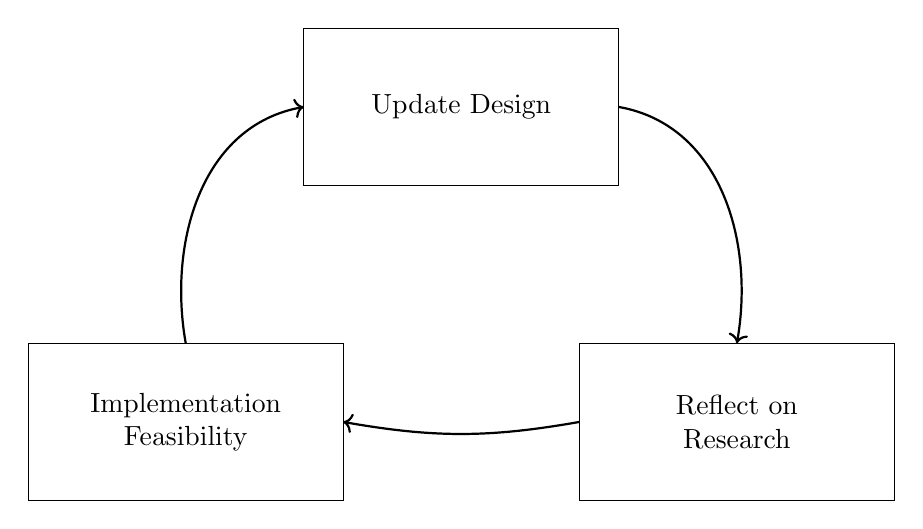
\begin{tikzpicture}
        \node[align=center] at (5.5,5) {Update Design};
        \draw (3.5,4) rectangle (7.5,6);

        \node[align=center] at (2,1) {Implementation\\Feasibility};
        \draw (0,0) rectangle (4,2);

        \node[align=center] at (9,1) {Reflect on\\Research};
        \draw (7,0) rectangle (11,2);

        \path (2,2) edge [->,thick,out=100,in=190]  (3.5,5);
        \path (7.5,5) edge [->,thick,out=350,in=80]  (9,2);
        \path (7,1) edge [->,thick,out=190,in=350]  (4,1);
      \end{tikzpicture}
    \caption{Iterative steps when designing for functional requirements}\label{figure:design-process}
  \end{figure}

  \section{Haar Engine}
    The first component to get design attention is the Haar Engine. The purpose of this framework is to provide the tools which enable developers to implement an IoT application. Since this will support the main system functions required for an IoT system applications, its design is heavily informed by the technologies available.

    One major design decision is the programming environment used to implement the Haar Engine. First of all, the chosen programming language and ecosystem must be able to support the requirements outlined in the previous chapter. Beyond that, the language and framework must provide suitable constructs so application developers can easily extend and modify for their own needs. Various languages and architectures were investigated (such as PHP, Ruby, Python and Go), however one stood out as being most suitable for this project, given the constraints: server-side JavaScript in the form of Node.js.

    JavaScript and the Node.js ecosystem will be discussed in greater detail in the implementation chapter, however there are some language features which are pertinent to the design of the framework. First of all, JavaScript is a weakly-typed, dynamic programming language. It does not support interfaces or abstract classes like Java, and variables are not defined with strict values. Care should therefore be taken when modelling system components as objects. JavaScript itself operates using the so-called event loop and all operations are considered asynchronous. Care should therefore be given to function executions, callbacks and the required call order.

    Node.js is a server-side implementation of the Google V8 JavaScript engine and it provides a programming API. There are various web application frameworks developed on top of Node.js, with the de facto standard being Express. The Express framework is based on the concept of middleware, where middleware functions anonymously pass objects to the next one until a web request has been finished. This concept could therefore be used to an advantage for system aspects like authentication.

    Bearing these language features in mind, a final design for the framework has been defined. A logical view of the main system components can be seen in Figure \ref{figure:framework-architecture}. The design decisions for each of these framework components have been described in the following subsections.

    \begin{figure}
    \centering
      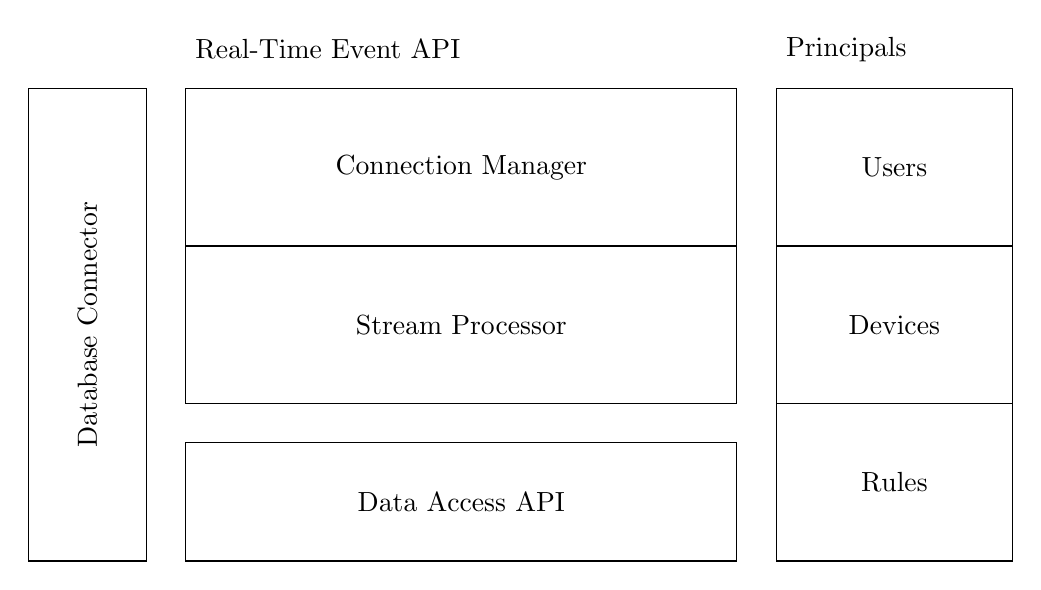
\begin{tikzpicture}
        \draw (0,0) rectangle (1.5,6);
        \node[align=center, rotate=90] at (0.75,3) {Database Connector};

        \draw (2,2) rectangle (9,6);
        \draw (2,4) -- (9,4);
        \node[anchor=west] at (2,6.5) {Real-Time Event API};
        \node[align=center] at (5.5,5) {Connection Manager};
        \node[align=center] at (5.5,3) {Stream Processor};

        \draw (2,0) rectangle (9,1.5);
        \node[align=center] at (5.5,0.75) {Data Access API};

        \draw (9.5,0) rectangle (12.5,6);
        \draw (9.5,4) -- (12.5,4);
        \draw (9.5,2) -- (12.5,2);
        \node[anchor=west] at (9.5,6.5) {Principals};
        \node[align=center] at (11,5) {Users};
        \node[align=center] at (11,3) {Devices};
        \node[align=center] at (11,1) {Rules};
      \end{tikzpicture}
    \caption{A logical view of system architecture for the Haar Engine}\label{figure:framework-architecture}
  \end{figure}

    \subsection{Data Modelling}
      The functional requirements in Chapter \ref{Chapter:Specification} make reference to a number of modellable objects. In particular these are users, devices and rules, and they all have a notion of ownership and authorisation within the framework. During initial research, it was found that an existing platform (Nitrogen.io) abstracts similar objects into a collection called principals. Throughout the design process, users, devices and rules have have proven to be first-class citizens of the framework, so the Haar Engine will adopt the same terminology.

      The three principal objects set foundations for the complete data model as well as other framework components, so it is important that they are modelled correctly. This subsection will first describe the traits of each principle before expanding their relationships into an entity-relationship model. Figure \ref{figure:principal-models} illustrates the relationship between the principals.

      \subsubsection{Users}
        The user principal is fundamentally responsible for authorisation within the Haar Engine. This will model an end-user account such as an individual person or a company, who will access their account using a unique username and a password. The user is responsible for managing their own devices and rules. The Haar Engine will identify user principals with a unique identifier. This would allow users to change their username while maintain relationships with other principals.

        User principals will be the gatekeeper to devices associated with their account. First of all, they will be able to attach new devices to their account. Users will also have the ability to share access to sensor devices with specific users, or make that data publicly available. Finally, user principals will have the ability to transfer ownership of the device to another Haar Engine user account and relinquish administration control over it.

        User principals will also be able to create, modify and delete rules. When a new rule is created, the user will be designated as the owner of it. Unlike devices, users cannot share rules with another user, nor can they transfer ownership. It is foreseeable that a rule is configured to watch sensor data which is owner by another user. Since access to a third-party sensor cannot be granted, the rule would not have appropriate access permissions to run.

      \subsubsection{Devices}
        The device principal will model a single IoT device. The device can be one of two types (either a sensor or an actuator). Devices will be owned by one user, however further users may be granted access to access sensor data. Devices will be identifiable with a unique identifier in the Haar Engine. This identifier will be used for the purpose of authentication and authorisation against user principals.

        The device model will also describe the type of data which it supports. For sensor devices, the principal will note the type of measurement (a single value or a vector of values) and the unit(s) of measurement. In the case of actuators, the principal will describe possible output types (single value or a vector of values), as well as value limits. These data type descriptions will be used when defining rules.

      \subsubsection{Rules}
        Rule principals define triggers within the Haar Engine. They are created and owned by a user principal. A rule will consist of a watch target, trigger criteria (such as threshold values), an action target and an action. The watch target is a sensor to monitor and when changes are detected, its output values will be compared against trigger criteria. If the criteria is met, the action target (actuator) will be updated in accordance with the action to take. The rules may run infinitely or they may be configured with a start and end date.

      \subsubsection{Entity Relationship Model}
        1. Entity Relationship Diagram using Bachman Notation.

        \begin{figure}[H]
        \centering
          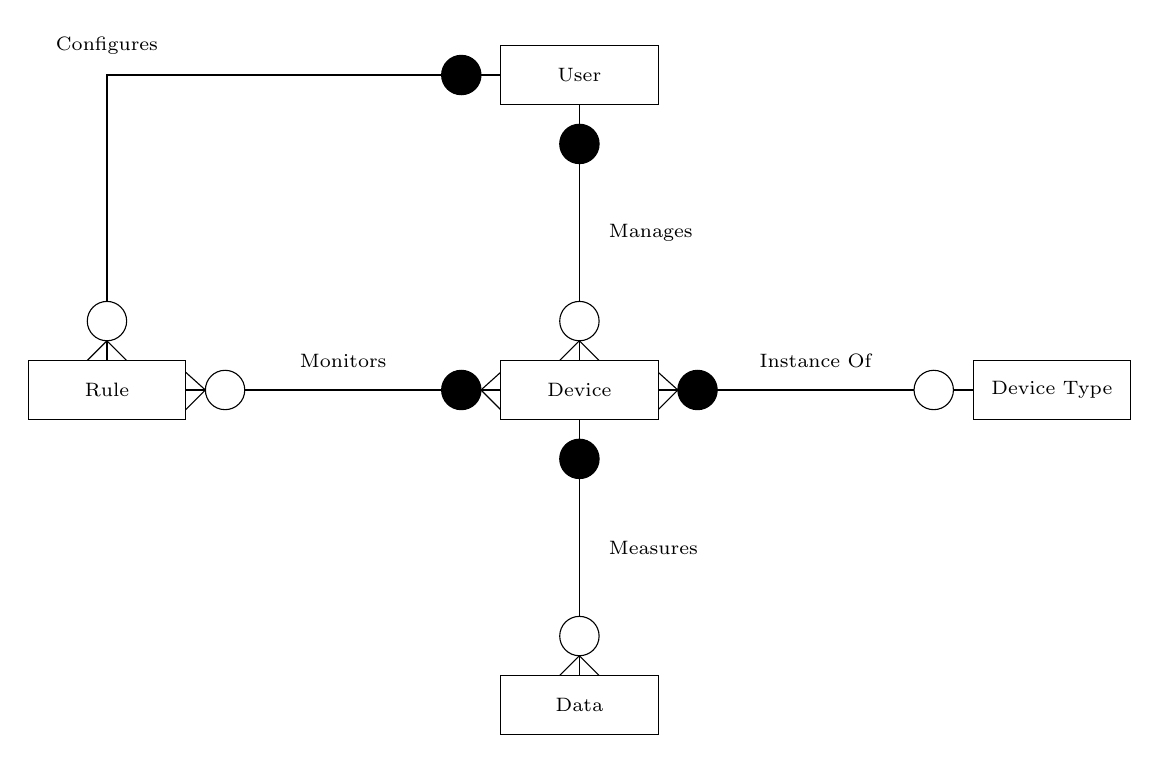
\begin{tikzpicture}
            \tikzstyle{every node}=[font=\scriptsize]

            \draw (7,8) -- (7,0.75);
            \draw (2,4.375) -- (12,4.375);
            \draw (1,4.75) -- (1,8.375) -- (6,8.375);

            \draw[fill=white] (2.5,4.375) circle [radius=0.25];
            \draw (2,4.6) -- (2.25, 4.375) -- (2,4.125);
            \node at (4,4.75) {Monitors};
            \draw (6,4.6) -- (5.75, 4.375) -- (6,4.125);
            \draw[fill=black] (5.5,4.375) circle [radius=0.25];

            \draw[fill=black] (8.5,4.375) circle [radius=0.25];
            \draw (8,4.6) -- (8.25, 4.375) -- (8,4.125);
            \node at (10,4.75) {Instance Of};
            \draw[fill=white] (11.5,4.375) circle [radius=0.25];

            \draw[fill=white] (7,5.25) circle [radius=0.25];
            \node[anchor=west] at (7.25,6.375) {Manages};
            \draw (6.75,4.75) -- (7, 5) -- (7.25,4.75);
            \draw[fill=black] (7,7.5) circle [radius=0.25];

            \draw[fill=black] (7,3.5) circle [radius=0.25];
            \node[anchor=west] at (7.25,2.375) {Measures};
            \draw (6.75,0.75) -- (7, 1) -- (7.25,0.75);
            \draw[fill=white] (7,1.25) circle [radius=0.25];

            \draw[fill=black] (5.5,8.375) circle [radius=0.25];
            \node at (1,8.75) {Configures};
            \draw (0.75,4.75) -- (1, 5) -- (1.25,4.75);
            \draw[fill=white] (1,5.25) circle [radius=0.25];

            \draw (0,4) rectangle (2,4.75);
            \node at (1,4.375) {Rule};

            \draw (6,0) rectangle (8,0.75);
            \node at (7,0.375) {Data};

            \draw (12,4) rectangle (14,4.75);
            \node at (13,4.375) {Device Type};

            \draw[fill=white] (6,4) rectangle (8,4.75);
            \node at (7,4.375) {Device};

            \draw (6,8) rectangle (8,8.75);
            \node at (7,8.375) {User};

          \end{tikzpicture}
        \caption{Entity Relationship Diagram for the Haar Engine}\label{figure:principal-models}
      \end{figure}

      2. Entity Sets
      \begin{itemize}
        \item User(\underline{id}, username, password, role)
        \item Device(\underline{id})
        \item Device Type(\underline{id}, type, structure)
        \item Data(\underline{id}, values)
        \item Rule(\underline{id}, watch target, criteria, action target, action)
      \end{itemize}

      3. Relationships
      \begin{itemize}
        \item Manages --- User manages Device [1:m][m:o]
        \item Configures --- User configures Rule [1:m][m:o]
        \item Instance Of --- Device instance of Device Type [m:1][o:m]
        \item Measures --- Device measures Data [1:m][m:o]
        \item Monitors --- Rule monitors Device [m:1][o:m]
      \end{itemize}

      4. Constraints and Assumptions
      \begin{itemize}
        \item Device Type structure is an array of objects. Each object describes a possible measurement.
        \item The Device Type of a device will never change
      \end{itemize}
    \subsection{Database Connector}
      Efficient data storage is an important performance consideration. The requirements in Chapter \ref{Chapter:Specification} also state that application developers should have the ability to change the database type to suit their own application. The design solution arrived at for this requirement is a database connector API.

      The database connector API will provide a set of foundation methods for operating on principal models and data generated by devices. The framework will use a consistent programming interface and this will allow application developers to change the connector for one of their own design. In a more strictly-typed programming language, object-oriented constructs such as abstract classes or interfaces might be used to define class signatures. With JavaScript, programming techniques like function composition might be more appropriate. 

      Whilst the Haar Engine will provide the capability of changing the database connector, an `out of the box' connector will be provided. A NoSQL database fits the purpose of the framework better than an SQL-based database because the data stored could be of varying formats and structures. There are a variety of NoSQL databases available, which will be discussed in the implementation chapter.

    \subsection{Data Access API}
      There are a number of mature standards used for structured data access on the web, so this requirement of the project is about choosing the most appropriate. Two widely-used access standards are Simple Object Access Protocol (SOAP) and Representational State Transfer (REST). These standards also use data interchange formats such as eXtensible Mark-up Language (XML) or JavaScript Object Notation (JSON).

      A REST API was found to be a better fit than SOAP for the Haar Engine. The REST access operators integrate much easier with potential implementation technologies like Node.js and Express and it is a simpler standard to use. The JSON data interchange format is based on JavaScript object constructs so it naturally integrates with a JavaScript-based application.

      Authentication will have to be enforced by every component of the Haar Engine, including the Data Access API. One characteristic of REST APIs is that they are stateless, meaning no session data is stored server-side and that every request will have to be inspected for appropriate access permissions. Two authentication techniques which will be used are a username and password combination, as well as token-based authentication. Clients will first authenticate with their username and password and if accepted, the REST API will return a unique access token for use in subsequent requests.

    \subsection{Real-Time Event API}
      One main characteristic of IoT is the ability to react on sensor data in real-time. This makes a robust and effective real-time API a priority for any given application. Giving structured access to this feature is challenging due to the points described in Section \ref{bidirectioncomms}. For this reason, the problem has been divided into two constituent components: opening and maintaining a true bidirectional communication channel, and efficiently handling messages between the two nodes of the channel.

      One technology which goes some distance in helping with this is MQTT. As described in Section \ref{section:mqtt}, MQTT is a publish-subscribe protocol which facilitates the transmission of messages. MQTT is a very robust protocol however given project constraints and additional the additional complexity which it might create, it has been deemed unfeasible for this project. Instead, the JavaScript project Socket.io can open and maintain WebSocket connections, with fallbacks if the WebSocket protocol is unavailable. The message-passing concepts of MQTT could be applied to Socket.io.

      \subsubsection{Connection Manager}
        The connection manager is responsible for navigating potential network issues to maintain a bidirectional communication channel. Choosing to use Socket.io and the WebSocket protocol should alleviate any of the issues regarding firewalls and NAT. Socket.io provides an API for managing WebSocket connections. Clients can connect to namespaced URIs which encapsulate different categories of client---the Haar Engine will use two default namespaces: sensors and actuators.

        It is also the responsibility of the connection manager to authenticate clients, whether they are users or devices. Socket.io also solves this problem with the use of its own middleware capability. This middleware could make use of authentication mechanisms already in place for the Data Access API.

      \subsubsection{Stream Processor}
        Once a connection has been established, it is the responsibility of the stream processor to act on messages. The Socket.io API allows clients to join one or more rooms within a given namespace and this capability will be leveraged by the stream processor. For example, multiple sensors will each have their own room under the sensor namespace. The stream processor can listen for any sensor events and store the data. Alternatively, stream processing rules (based on the rule principal object) could listen for messages in a single sensor room and act accordingly.

  \section{Haar}
    The main purpose of the second component, Haar, is to validate the implementation of the Haar Engine. Most of the heavy lifting will be done by the Haar Engine, however this application also requires design attention, especially in regards to the end devices. There are three main components to be investigated: the back-end application, front-end application (dashboard) and the wireless sensor network itself. Figure x.x. illustrates the relationship between these components.

    \subsection{Back-End Application}
      The back-end application is simply an instance of the Haar Engine. It is expected that the data models will be extended for one or two application-specific fields (such as a profile picture and biography for users) however it will generally be left as designed. The back-end application will be self-contained and separate from the front-end application. 

    \subsection{Front-End Application}
      The front-end application is, in essence, simply a user interface for the back-end APIs. It will make use of the Data Access API and Real-Time Event API to manage users, devices, rules and the authentication for all of them. The main challenge presented by the dashboard is handling very dynamic, real-time data in a structured and efficient way for a variety web browsers. The implementation details of this will be discussed in detail as part of the next chapter.

      What can be discussed at this stage is the design, layout and behaviour of the user interface. Figure \ref{figure:desktop-layout} illustrates the general layout which will be used. On desktop-sized web browsers, the window will be split into two panes---one used for navigation, and one for displaying the current page content. On mobile-sized web browsers, only one pane will be displayed at a time. By default, this will be the content pane and when the navigation button is clicked, the navigation pane will be shown.

      The behaviour of the user interface is a challenging aspect. It is expected that aspects of the user interface will react in real-time to new data, so it will also have to open a connection to the Real-Time Event API. This will be possible by using the Socket.io library client-side. The challenges begin when the user starts to navigate to different pages of the dashboard. Traditionally this would load a completely new page, however real-time connections would have to be renegotiated and this is inefficient. Instead, dashboard pages will be loaded asynchronously. Care must then be taken to achieving this in a structured way with in its implementation.

      \begin{figure}
        \centering
          \begin{tikzpicture}
            \node[inner sep=0pt] at (0,0)
              {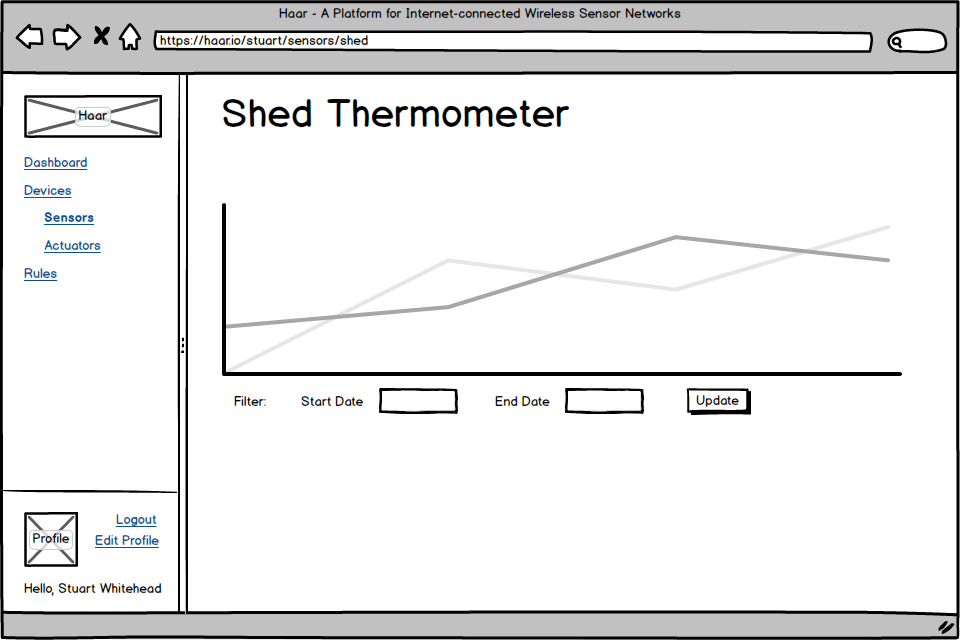
\includegraphics[width=\textwidth]{assets/desktop-layout.png}};
          \end{tikzpicture}
        \caption{UI layout for desktop-sized web browsers}\label{figure:desktop-layout}
      \end{figure}

    \subsection{Wireless Sensor Networks}
      The third and final component for the Haar application is the wireless sensor network. The wireless sensor network comprises of the physical sensors and actuators which create an interface between the physical and digital worlds. To fully demonstrate the capability of the Haar Engine, there is a requirement for a variety of sensor types.

      \subsubsection{Bridge}
        % Maintain communication channel
        % Map messages to and from nodes

      \subsubsection{End Devices}
        % Low-power nodes
        % Constrained processing power
    \chapter{Development Practices}
  A software implementation can be set up for success or failure before any code has been written, especially whilst working within a team. This is down to the development process and policies in place. Of course, one process may work for one team or project and not another.

  A well implemented process can provide many benefits. First and foremost, everyone in a development team clearly understands their roles and responsibilities. The process can also enforce a hierarchy of decision making, or encourage peer collaboration. Beyond these people-based benefits, a development process can aid in the development of a robust, maintainable codebase. A developer who can understand a codebase and make confident updates is an efficient one.

  Although the output of this project is the work of one person, arguments supporting a process-first implementation still apply. The following section will detail the main tools used in supporting this project. 

  \section{Version Control System}
    The use of a Version Control System (VCS) is highly recommended in any project. As the name suggests, a VCS manages iterative updates of project files. To generalise its functionality, a VCS maintains a timeline of file states. Different states of the same file can be compared to investigate which changes were made and by whom, and if needed a file can be reverted to a previous state. This means that the complete history of a codebase is recorded. Without using a VCS, code updates would simply overwrite the existing file and old states would be lost forever.

    There are a number of Version Control Systems available to developers, such as Mercurial and Subversion. Git is another VCS and was created by Linus Torvalds, creator and maintainer of the Linux kernel. Git is arguably the most popular VCS amongst the open source community, thanks to its use in the development of the Linux kernel. Its command-line interface is highly portable and many community-oriented services support it extensively, such as GitHub and Bitbucket.

    Git along with the web-based service GitHub have been chosen for use in this project thanks to their universal support. But simply selecting a tool is not enough when implementing a development process - guidelines on how to use it should also be decided. There are a number of well-defined development workflows using Git. This project has chosen to implement the `Git Flow' workflow. Git Flow utilises various features of Git and GitHub, including branching, merging and pull requests. 

    Describing the Git and the Git Flow workflow could fill an article on its own, so this description will be very brief. In Git, a branch is an instance of the complete codebase. Multiple branches with different versions of the same codebase can be developed in parallel. The merge command copies the changes of one branch into another. A Pull Request is a request to merge one branch into another, which can be inspected and commented on before the merge is completed.

    The Git Flow workflow adds structure to these features. The master branch is the production codebase. The develop branch is the in-progress codebase. Feature branches (such as feature/menu or feature/users-controller) are used to develop a specific feature of the project. Once the feature has been built, a pull request is raised to merge it into the develop branch. Once all features have been merged and tested, a pull request is raised to merge the develop branch into master which is then deployed. This workflow has been employed for this project.

    \subsection{Pre-commit Hook}
    \label{section:pre-commit-hook}
      The Git VCS also supports lifecycle hooks. These hooks allow developers to run bespoke scripts to enforce custom policies, such as limiting access to specific branches. One helpful trick has also been employed for this project through the use of the pre-commit hook.

      No matter how descriptive or strict development policies are, developers are only human. Humans can make mistakes and they can be lazy, meaning that poor quality code can be committed to the codebase. The pre-commit hook can be used to enforce a specific coding standard. It works by testing the committed code against a set of rules. If the tests pass, the code is committed to the codebase but if they fail, a warning message is displayed. By using this technique, the code for this project is guaranteed to be of a certain standard.

  \section{Docker}
  \label{section:docker}
    Developers face a number of challenges when developing and deploying modern web-based applications. Primarily, the environment in which code is executed can differ wildly. For any given project, one developer might use a Windows machine whilst their colleague could use an Apple Mac. The staging environment could use one version of Linux whereas the production environment could use another. All of these environments could potentially run differing versions of the same software meaning that bugs in the project might not be traceable or reproducible. Development teams have attempted to normalise these environments through the use of package managers, however these still leave room for misconfiguration.

    A relatively new tool called Docker has been taking the development world by storm since its release in 2013. Docker builds on a technology called Linux Containers. Traditional virtual machines run a complete operating system (kernel, program binaries and any other files) on top of a host machine. In comparison, Docker (and Linux Containers) allow images to use the same kernel of the host operating system. This means that each container is very lightweight but can still benefit from the complete isolation of program processes.

    Docker containers are instances of a Docker image. Docker images are compiled according to a Dockerfile which comprise of commands such as COPY (to copy source files to the image) and RUN (to run Unix commands within the Linux Container). This is where the advantages of Docker become clear - explicit, reproducible environments can be built as if working directly on a server. Since Docker is a portable tool, every developer working on a project can run exactly the same environment as each other. When the application is ready to be deployed, the same Docker image can be executed on a production server.

    Docker also has powerful composition tools. Anything beyond a simple script or application is typically the sum of many smaller, more specific applications. A simple example of this would be a dynamic web application backed by a database. In Docker terms, this application would be composed of two images - one image for the dynamic web application, and another for the database. Docker can configure automatic links between instances of these images and this is aided with the helped command-line interface `docker compose'.

    Docker Compose makes use of another configuration file, `docker-compose.yml'. In this file it is possible to specify which Docker images make up a complete application (which can be custom builds using a Dockerfile, or pre-built images from the global Docker repository). Using this file Docker Compose will intelligently start Docker images in order of their dependencies. Using the dynamic web application and database example, the database would be started first and then the application. Docker will also set up lots of other clever tools, such as a long list of environment variables referring to specific links. These environment variables can then be used within applications to configure things like database connections.

    Once applications have been wrapped up into Docker images and compositions, it is then necessary to deploy them to servers. This can of course be achieved manually using the docker CLI, however the Docker ecosystem also includes Docker Cloud, a first-party container deployment service. Docker Cloud uses four more important terms to describe an application:

    \begin{description}
      \item[Node] a server which can host Docker containers
      \item[Node Cluster] a grouping of multiple servers which can host Docker containers
      \item[Service] one or more running container instances of a Docker image
      \item[Stack] an application composed of multiple services
    \end{description}

    Docker Cloud is very simple but hugely powerful. Scaling is an important aspect of any web application and is handled with grace. Docker Cloud will intelligently distribute container instances across all available nodes based on their loads. It will then lay a private network between all services of a stack (irrespective of its host node) so all containers can transparently communicate. This makes load balancing truly simple.

    Docker has been chosen as a critical piece of infrastructure for this project. Flexibility, robustness and maintainability are three important aspects when developing any application and Docker aids these areas very effectively.

  \section{Continuous Integration}
    The development process has so far defined how the codebase will be developed and how it will be hosted, but there is still an important step missing. How does newly developed code get deployed in a way which ensures no downtime and without bugs? This is where a technique called Continuous Integration (CI) is used.

    Continuous Integration is the glue between the processes at each end of the development cycle. The main ethos behind it is to deploy little and often. This allows developers to catch issues early and to pin-point its cause quickly. \citet{continuous-integration} describe CI with a number of key points, including: automated, self-testing builds and automated deployments. As it turns out, the Git Flow workflow, Docker and Continuous Integration all work incredibly well together.

    As has already been discussed, Docker images provide explicit, reproducible environments and this is great for testing purposes. Since all Docker environments will be built equal, it means tests run on a local machine will behave the same on a production server. And because Docker Compose can specify which images needs to be used, any service with access to this information can build the correct application dependencies.

    Travis CI is one such continuous integration service which supports the Docker ecosystem. It has been employed in this project to enforce a CI workflow and it follows these steps:

    \begin{enumerate}
      \item Code is developed using the Git Flow workflow
      \item All commits to branches and pull requests trigger tests on Travis CI
      \item Each test builds the Docker environment to ensure consistency
      \item If tests pass, the Docker image is published to the Docker repository
      \item The Docker repository will deploy new images through Docker Cloud
    \end{enumerate}

    This workflow contributes to a solid development process which can be scaled to a large codebase and team of developers.
    \input{mainmatter/implementation}
    \chapter{Results and Evaluation}
    \chapter{Conclusions}
  To recap, this project specified four main objectives in order to satisfy three high-level aims. The objectives were to research IoT practices and concepts; to research supporting technologies; to develop an IoT application framework and to develop a demonstration application using the framework. These objectives have been successfully achieved.

  This chapter will discuss the main lessons learnt during the course of the project. This discussion will cover the current state of the Internet of Things and the challenges it still faces. Additionally, topics of future work will be discussed based on the challenges uncovered. Finally, this chapter will critically appraise my conduct for the project and I will give a brief personal reflection of the honours experience.

  \section{The Internet of Things}
    The easiest conclusion to draw about IoT is that it is an unsettled area of research. The diversity of research shows that academic institutions and manufacturers are investing a lot of time and money into the concept. They are motivated to do so by the potential opportunities lying in wait, like smart cities and the connected home. Undoubtably there are many use cases which have not yet been imagined.

    One downside to the volume of research being conducted is the increasingly fragmented array of technologies available. In some cases there are numerous competing technologies which address the same challenge, such as the various implementations of the IEEE 802.15.4 Low-Rate Wireless Personal Area Networks standard. ZigBee and 6LowPAN are only two of many 802.15.4 implementations. It would appear that the IoT concept is now at a consolidation stage where best practices and go-to technologies will identified.

    Some technologies are already emerging as a standard tool for IoT applications. The frameworks and platforms investigated in Chapter \ref{Chapter:Background} (Background) support a variety of connectivity protocols and techniques, including HTTP, UDP single-shot, CoAP and MQTT. HTTP is already established as the \textit{de facto} Internet communication protocol, making it the ideal choice for the distribution of meta and configuration data for IoT applications. HTTP however lacks the mechanisms to facilitate real-time, bidirectional event streams. MQTT is emerging as the technology of choice for this purpose as indicated by Amazon's support for it.

    A final conclusion to draw on IoT is that it is a truly multidisciplinary concept. Successful IoT applications will rely on an effective collaboration between computer scientists, designers, user researchers and engineers. Organisations like Google, Amazon and Samsung will strive in the respect because they have access to the necessary expertise and already implement mature product development processes. The user experience is a crucial aspect to get right; the best IoT applications will be those which are invisible or second-nature to its users.

  \section{Future Work}
    There remains a lot of work to complete in the realm of IoT. One of the challenges not addressed in this project was the association of IoT devices to other devices and networks. There were eight XBee radio chips used across two ZigBee networks for the Haar demonstration application. These devices and networks were all configured through a manual and laborious process; an process which is not possible for the average consumer. So how, then, can constrained devices with little or no human-computer interaction be set up? Maybe Near Field Communication (NFC) could be used to configure network settings of nearby devices. This is as a much a challenge for product designers as it is for computer scientists.

    The unfortunate necessity for a bridge device is another aspect to be addressed. The bridge device is in essence a router to translate data between the Internet and wireless smart devices. As was described in Section \ref{bidirectioncomms}, the configuration of the Local Area Network and its firewall can also impact the available technologies. There is potentially a market for a smart network hub which integrates traditional networking components like a router, firewall and a WiFi access point with IoT-specific technologies like an IEEE 802.15.4 radio transceiver. A `Smart Home Hub' such as this could facilitate the association of IoT devices and their network requirements.

    Haar Bridge is a response to what is the most pronounced challenge in facilitating end-to-end global connectivity for IoT devices. The Internet infrastructure relies on the TCP/IP protocol but this is, in large, not compatible with the optimised wireless communication protocols implemented in constrained devices. Some protocols like ZigBee IP and 6LoWPAN attempt to extend TCP/IP compatibility but there is still work to be done. In particular, these protocols rely on IPv6 and the uptake of this has been slow.

  \section{Critical Appraisal}
    Overall I am satisfied with my conduct and the I effort put into this project. I feel that I have worked to the best of my ability and made the best use of the time available. The time spent working on the implementation is small when compared to the time spent researching and designing; as an estimate, one-third of the time was spent on implementation whereas two-thirds of the time was spent reading, designing, writing and evaluating.

    One improvement which could be improved is the approach to user research and evaluation. This project was very much driven by the momentum in the IoT area; the implementation was based on a consolidation of the emerging IoT practices and technologies. Future projects could perform user research to determine which features of a framework would be the most useful, for example. External users could then be used in order to evaluate the effectiveness and flexibility of the software.

    For me, the most difficult aspect of the whole project was at the design stage. It took many design iterations to arrive at a solution which both satisfied the information uncovered in Chapter \ref{Chapter:Background} and was feasible to implement. I think that the difficulty came from the fact that IoT is still an immature area and that there are few established practices already in place.

    Going into this project, I had a curiosity in the Internet of Things but not an active interest. Now that the project has been completed, I would say that I am now more interested in the field and would be keen to continue learning about this subject. I think the implementation and the potential it demonstrates has also captured the interest of other students, lecturers and work colleagues. That is what I am most proud of.


  \appendix
    \chapter{Haar Engine Acceptance Tests}
  \begin{longtabu} to \textwidth {|X|c|X|}
    \hline
      \textbf{Requirement}
      & \textbf{Status}
      & \textbf{Notes}
    \endhead \hline
      The framework shall model users
      & Implemented
      &
    \\ \hline
      A user shall be identified by a unique username
      & Implemented
      &
    \\ \hline
      A user shall have an associated profile including: full name, email address
      & Implemented
      &
    \\ \hline
      Users shall be assigned a privilege level: standard or administrator
      & Implemented
      & Haar Engine understands privileges as `user' or `admin'
    \\ \hline
      The framework shall authenticate genuine users only
      & Implemented
      & Implemented with a combination of user credentials, Bcrypt password hashing and signed JSON Web Tokens
    \\ \hline
      The framework shall model connected IoT devices
      & Implemented
      &
    \\ \hline
      A device shall be identified by a unique identification number
      & Implemented
      & Devices are assigned a random, unique ID for use in data modelling. Haar Engine also stores their globally unique MAC address.
    \\ \hline
      A device shall be designated as either an input (sensor) or output (actuator)
      & Implemented
      &
    \\ \hline
      The framework shall authenticate genuine devices only
      & Implemented
      &
    \\ \hline
      The framework shall authorise and facilitate the management of devices
      & Implemented
      &
    \\ \hline
      A device will have one owner
      & Implemented
      &
    \\ \hline
      Access to device data and configuration options shall be restricted to the device owner by default
      & Implemented
      & This feature is restricted solely to the device owner and cannot be delegated.
    \\ \hline
      The device owner shall be able to make device data public
      & Implemented
      &
    \\ \hline
      A device owner shall be able to grant access permission to specified users
      & Not Implemented
      &
    \\ \hline
      The framework shall establish a connection with end devices
      & Implemented
      &
    \\ \hline
      Devices shall be addressable and identifiable whilst the connection is open
      & Implemented
      & Through the use of a publish/subscribe architecture
    \\ \hline
      The connection shall remain open under normal operating conditions
      & Implemented
      &
    \\ \hline
      Under error conditions, the connection shall be re-established
      & Implemented
      & Facilitated through the Primus real-time library
    \\ \hline
      The connection shall be bidirectional
      & Implemented
      & Implemented with WebSockets, supported by the Primus real-time library
    \\ \hline
      Input devices shall be able to transmit data packets to the framework
      & Implemented
      &
    \\ \hline
      The framework shall be able to transmit data packets to output devices
      & Implemented
      &
    \\ \hline
      The connection shall be tolerant of network obstacles such as firewalls and Network Address Translation
      & Implemented
      &
    \\ \hline
      The framework shall store data received by devices
      & Implemented
      &
    \\ \hline
      The framework shall provide an interface for using different database types
      & Not Implemented
      & Only one database type is supported: MongoDB. Its implementation is however extensible and allows developers to modify schemas.
    \\ \hline
      The framework shall provide a default ‘out of the box’ database connector
      & Implemented
      & There is only one.
    \\ \hline
      Application developers shall be able to create their own database connectors
      & Not Implemented
      &
    \\ \hline
      The framework shall provide structured access to stored data
      & Implemented
      &
    \\ \hline
      Access shall be granted to authenticated and authorised users only
      & Implemented
      &
    \\ \hline
      Application developers shall be able to modify data access
      & Implemented
      & Developers have the opportunity to implement new controllers or override existing
    \\ \hline
      Application developers shall be able to add custom data searches
      & Implemented
      & Developers have the opportunity to implement new controllers or override existing
    \\ \hline
      Application developers shall be able to add custom data filters
      & Implemented
      & Developers have the opportunity to implement new controllers or override existing
    \\ \hline
      The framework shall provide a real-time event API
      & Implemented
      & Based on MQTT's publish/subscribe model
    \\ \hline
      Client applications shall be able to listen for device events
      & Implemented
      &
    \\ \hline
      The real-time API shall leverage bidirectional connectivity with devices
      & Implemented
      &
    \\ \hline
      The API shall provide real-time access to data received from devices
      & Implemented
      &
    \\ \hline
      The real-time API shall enable developers to create application rules and triggers
      & Implemented
      &
    \\ \hline

    \caption{User Acceptance Testing for Haar Engine}\label{haar-engine-acceptance}
  \end{longtabu}
    \chapter{Haar Acceptance Tests}
\ref{chapter:haar-acceptance}
  \begin{longtabu} to \textwidth {|X|c|X|}
    \hline
      \textbf{Requirement}
      & \textbf{Status}
      & \textbf{Notes}
    \endhead \hline
      The application shall comprise of two local area device networks
      & Implemented
      & 
    \\ \hline
      Devices of these networks shall be capable of establishing a connection between themselves and the web application
      & Implemented
      & This is facilitated through the bridge device
    \\ \hline
      The device networks shall comprise of two sensor devices
      & Implemented
      & Network A comprises temperature and RGB colour sensors; Network B comprises temperature and gyroscope sensors
    \\ \hline
      The device network shall contain a sensor device which measures a single data point, such as temperature
      & Implemented
      & Implemented in the form of a temperature sensor
    \\ \hline
      The device network shall contain a sensor device which measures more complex data, such as a vector of wind direction and speed
      & Implemented
      & Implemented in the form of RGB colour sensor (red, green and blue values) and gyroscope sensor (x, y and z values)
    \\ \hline
      The device networks shall comprise of a single actuator device
      & Implemented
      & Implemented as an RGB LED lamp
    \\ \hline
      The actuator device shall be flexible enough to represent a variety of data types
      & Implemented
      &
    \\ \hline
      The web-based dashboard will be the main interface between a user and their devices.
      & Implemented
      &
    \\ \hline
      The dashboard shall be accessible on the World Wide Web
      & Implemented
      & Hosted using DigitalOcean cloud server
    \\ \hline
      The dashboard shall authenticate users with a username and password
      & Implemented
      &
    \\ \hline
      The dashboard shall list profile details
      & Implemented
      &
    \\ \hline
      The user shall be able to manage their devices
      & Implemented
      &
    \\ \hline
      The dashboard shall list devices owned by the user
      & Implemented
      &
    \\ \hline
      The user shall be able to add a new device
      & Implemented
      &
    \\ \hline
      The dashboard shall show whether devices are connected or not
      & Not Implemented
      & Sensors have the ability to sleep and are therefore not `connected' all of the time, but are still active
    \\ \hline
      The user shall be able to transfer ownership of the device
      & Not Implemented
      & The required permission system to facilitate this is too involved given the time constraints
    \\ \hline
      The user shall be able to grant access permissions to other users
      & Not Implemented
      & The required permission system to facilitate this is too involved given the time constraints
    \\ \hline
      The dashboard shall enable users to manage application rules
      & Implemented
      &
    \\ \hline
      The dashboard shall list existing rules
      & Implemented
      &
    \\ \hline
      The user shall be able to create new rules
      & Implemented
      &
    \\ \hline
      An actuator device shall be able to react to sensed data
      & Implemented
      &
    \\ \hline
      User devices shall be able to integrate with third-party services
      & Implemented
      & Possible through the use of Data Access and Real-Time Event APIs
    \\ \hline
      The dashboard shall display data for a given device
      & Implemented
      &
    \\ \hline
      The dashboard shall be able to trigger actuators with virtual controls
      & Not Implemented
      & This `nice to have' was not implemented given time constraints
    \\ \hline
      A section of the dashboard shall be dedicated to data visualisation
      & Implemented
      &
    \\ \hline
      A generic visualisation tool shall plot temporal data as a graph
      & Implemented
      &
    \\ \hline
      The date range shall be configurable
      & Implemented
      &
    \\ \hline
      Multiple data sources shall be comparable on one graph interface
      & Partial
      & Multiple data points from a single device can be displayed (e.g. red, green and blue); the data from multiple devices cannot be compared
    \\ \hline
      The graph shall leverage the real-time event API to update when new data is received
      & Implemented
      &
    \\ \hline
      Specialised visualisation tools shall reflect specific device types. For example, a virtual thermometer would visualise a temperature
      & Not Implemented
      & This `nice to have' was not implemented given time constraints
    \\ \hline
      Specialised visualisation tools shall leverage the real-time event API to update when new data is received
      & Not Implemented
      & This `nice to have' was not implemented given time constraints
    \\ \hline

    \caption{User Acceptance Testing for Haar}
    \label{table:haar-acceptance}
  \end{longtabu}
    \chapter{Credits}
\label{chapter:credits}
  \section*{Async}
    \begin{description}
      \item[Maintainer] Caolan McHanon
      \item[Usage] Managing application concurrency for features like simultaneous database queries
      \item[License] \scriptsize Copyright (c) 2010-2016 Caolan McMahon

        Permission is hereby granted, free of charge, to any person obtaining a copy
        of this software and associated documentation files (the ``Software''), to deal
        in the Software without restriction, including without limitation the rights
        to use, copy, modify, merge, publish, distribute, sublicense, and/or sell
        copies of the Software, and to permit persons to whom the Software is
        furnished to do so, subject to the following conditions:

        The above copyright notice and this permission notice shall be included in
        all copies or substantial portions of the Software.

        THE SOFTWARE IS PROVIDED ``AS IS'', WITHOUT WARRANTY OF ANY KIND, EXPRESS OR
        IMPLIED, INCLUDING BUT NOT LIMITED TO THE WARRANTIES OF MERCHANTABILITY,
        FITNESS FOR A PARTICULAR PURPOSE AND NONINFRINGEMENT. IN NO EVENT SHALL THE
        AUTHORS OR COPYRIGHT HOLDERS BE LIABLE FOR ANY CLAIM, DAMAGES OR OTHER
        LIABILITY, WHETHER IN AN ACTION OF CONTRACT, TORT OR OTHERWISE, ARISING FROM,
        OUT OF OR IN CONNECTION WITH THE SOFTWARE OR THE USE OR OTHER DEALINGS IN
        THE SOFTWARE.
    \end{description}

  \section*{Axios}
    \begin{description}
      \item[Maintainer] Matt Zabriskie
      \item[Usage] Universal, promise-based HTTP request library
      \item[License] \scriptsize Copyright (c) 2014 Matt Zabriskie

        Permission is hereby granted, free of charge, to any person obtaining a copy
        of this software and associated documentation files (the ``Software''), to deal
        in the Software without restriction, including without limitation the rights
        to use, copy, modify, merge, publish, distribute, sublicense, and/or sell
        copies of the Software, and to permit persons to whom the Software is
        furnished to do so, subject to the following conditions:

        The above copyright notice and this permission notice shall be included in
        all copies or substantial portions of the Software.

        THE SOFTWARE IS PROVIDED ``AS IS'', WITHOUT WARRANTY OF ANY KIND, EXPRESS OR
        IMPLIED, INCLUDING BUT NOT LIMITED TO THE WARRANTIES OF MERCHANTABILITY,
        FITNESS FOR A PARTICULAR PURPOSE AND NONINFRINGEMENT. IN NO EVENT SHALL THE
        AUTHORS OR COPYRIGHT HOLDERS BE LIABLE FOR ANY CLAIM, DAMAGES OR OTHER
        LIABILITY, WHETHER IN AN ACTION OF CONTRACT, TORT OR OTHERWISE, ARISING FROM,
        OUT OF OR IN CONNECTION WITH THE SOFTWARE OR THE USE OR OTHER DEALINGS IN
        THE SOFTWARE.
    \end{description}

  \section*{Babel (including helpers and plugins)}
    \begin{description}
      \item[Maintainer] Sebastian McKenzie
      \item[Usage] Compiling ES2015 syntax into ECMAScript 5
      \item[License] \scriptsize Copyright (c) 2014-2016 Sebastian McKenzie <sebmck@gmail.com>

        MIT License

        Permission is hereby granted, free of charge, to any person obtaining
        a copy of this software and associated documentation files (the
        ``Software''), to deal in the Software without restriction, including
        without limitation the rights to use, copy, modify, merge, publish,
        distribute, sublicense, and/or sell copies of the Software, and to
        permit persons to whom the Software is furnished to do so, subject to
        the following conditions:

        The above copyright notice and this permission notice shall be
        included in all copies or substantial portions of the Software.

        THE SOFTWARE IS PROVIDED ``AS IS'', WITHOUT WARRANTY OF ANY KIND,
        EXPRESS OR IMPLIED, INCLUDING BUT NOT LIMITED TO THE WARRANTIES OF
        MERCHANTABILITY, FITNESS FOR A PARTICULAR PURPOSE AND
        NONINFRINGEMENT. IN NO EVENT SHALL THE AUTHORS OR COPYRIGHT HOLDERS BE
        LIABLE FOR ANY CLAIM, DAMAGES OR OTHER LIABILITY, WHETHER IN AN ACTION
        OF CONTRACT, TORT OR OTHERWISE, ARISING FROM, OUT OF OR IN CONNECTION
        WITH THE SOFTWARE OR THE USE OR OTHER DEALINGS IN THE SOFTWARE.
    \end{description}

  \section*{Bcrypt}
    \begin{description}
      \item[Maintainer] Nick Campbell
      \item[Usage] Hashing and comparing user passwords
      \item[License] \scriptsize Copyright (c) 2010 Nicholas Campbell

        Permission is hereby granted, free of charge, to any person obtaining a copy
        of this software and associated documentation files (the``Software''), to deal
        in the Software without restriction, including without limitation the rights
        to use, copy, modify, merge, publish, distribute, sublicense, and/or sell
        copies of the Software, and to permit persons to whom the Software is
        furnished to do so, subject to the following conditions:

        The above copyright notice and this permission notice shall be included in
        all copies or substantial portions of the Software.

        THE SOFTWARE IS PROVIDED ``AS IS'', WITHOUT WARRANTY OF ANY KIND, EXPRESS OR
        IMPLIED, INCLUDING BUT NOT LIMITED TO THE WARRANTIES OF MERCHANTABILITY,
        FITNESS FOR A PARTICULAR PURPOSE AND NONINFRINGEMENT. IN NO EVENT SHALL THE
        AUTHORS OR COPYRIGHT HOLDERS BE LIABLE FOR ANY CLAIM, DAMAGES OR OTHER
        LIABILITY, WHETHER IN AN ACTION OF CONTRACT, TORT OR OTHERWISE, ARISING FROM,
        OUT OF OR IN CONNECTION WITH THE SOFTWARE OR THE USE OR OTHER DEALINGS IN
        THE SOFTWARE. 
    \end{description}

  \section*{Body Parser}
    \begin{description}
      \item[Maintainers] Jonathan Ong, Douglas Christopher Wilson 
      \item[Usage] Express middleware for parsing JSON and application/x-www-form-urlencoded request data into JavaScript object
      \item[License] \scriptsize (The MIT License)

        Copyright (c) 2014 Jonathan Ong <me@jongleberry.com>
        Copyright (c) 2014-2015 Douglas Christopher Wilson <doug@somethingdoug.com>

        Permission is hereby granted, free of charge, to any person obtaining
        a copy of this software and associated documentation files (the
        `Software'), to deal in the Software without restriction, including
        without limitation the rights to use, copy, modify, merge, publish,
        distribute, sublicense, and/or sell copies of the Software, and to
        permit persons to whom the Software is furnished to do so, subject to
        the following conditions:

        The above copyright notice and this permission notice shall be
        included in all copies or substantial portions of the Software.

        THE SOFTWARE IS PROVIDED `AS IS', WITHOUT WARRANTY OF ANY KIND,
        EXPRESS OR IMPLIED, INCLUDING BUT NOT LIMITED TO THE WARRANTIES OF
        MERCHANTABILITY, FITNESS FOR A PARTICULAR PURPOSE AND NONINFRINGEMENT.
        IN NO EVENT SHALL THE AUTHORS OR COPYRIGHT HOLDERS BE LIABLE FOR ANY
        CLAIM, DAMAGES OR OTHER LIABILITY, WHETHER IN AN ACTION OF CONTRACT,
        TORT OR OTHERWISE, ARISING FROM, OUT OF OR IN CONNECTION WITH THE
        SOFTWARE OR THE USE OR OTHER DEALINGS IN THE SOFTWARE.
    \end{description}

  \section*{Chart.js}
    \begin{description}
      \item[Maintainer] Nick Downie
      \item[Usage] Drawing charts for data pages
      \item[License] \scriptsize The MIT License (MIT) Copyright (c) 2013-2016 Nick Downie

        Permission is hereby granted, free of charge, to any person obtaining a copy of this software and associated documentation files (the ``Software''), to deal in the Software without restriction, including without limitation the rights to use, copy, modify, merge, publish, distribute, sublicense, and/or sell copies of the Software, and to permit persons to whom the Software is furnished to do so, subject to the following conditions:

        The above copyright notice and this permission notice shall be included in all copies or substantial portions of the Software.

        THE SOFTWARE IS PROVIDED ``AS IS'', WITHOUT WARRANTY OF ANY KIND, EXPRESS OR IMPLIED, INCLUDING BUT NOT LIMITED TO THE WARRANTIES OF MERCHANTABILITY, FITNESS FOR A PARTICULAR PURPOSE AND NONINFRINGEMENT. IN NO EVENT SHALL THE AUTHORS OR COPYRIGHT HOLDERS BE LIABLE FOR ANY CLAIM, DAMAGES OR OTHER LIABILITY, WHETHER IN AN ACTION OF CONTRACT, TORT OR OTHERWISE, ARISING FROM, OUT OF OR IN CONNECTION WITH THE SOFTWARE OR THE USE OR OTHER DEALINGS IN THE SOFTWARE.
    \end{description}

  \section*{Classnames}
    \begin{description}
      \item[Maintainer] Jed Watson
      \item[Usage] Build classname strings for React JavaScript components
      \item[License] \scriptsize The MIT License (MIT)

        Copyright (c) 2016 Jed Watson

        Permission is hereby granted, free of charge, to any person obtaining a copy
        of this software and associated documentation files (the ``Software''), to deal
        in the Software without restriction, including without limitation the rights
        to use, copy, modify, merge, publish, distribute, sublicense, and/or sell
        copies of the Software, and to permit persons to whom the Software is
        furnished to do so, subject to the following conditions:

        The above copyright notice and this permission notice shall be included in all
        copies or substantial portions of the Software.

        THE SOFTWARE IS PROVIDED ``AS IS'', WITHOUT WARRANTY OF ANY KIND, EXPRESS OR
        IMPLIED, INCLUDING BUT NOT LIMITED TO THE WARRANTIES OF MERCHANTABILITY,
        FITNESS FOR A PARTICULAR PURPOSE AND NONINFRINGEMENT. IN NO EVENT SHALL THE
        AUTHORS OR COPYRIGHT HOLDERS BE LIABLE FOR ANY CLAIM, DAMAGES OR OTHER
        LIABILITY, WHETHER IN AN ACTION OF CONTRACT, TORT OR OTHERWISE, ARISING FROM,
        OUT OF OR IN CONNECTION WITH THE SOFTWARE OR THE USE OR OTHER DEALINGS IN THE
        SOFTWARE.
    \end{description}

  \section*{Cookie Parser}
    \begin{description}
      \item[Maintainers] TJ Holowaychuk, Douglas Christopher Wilson
      \item[Usage] Express middleware for getting and and setting cookies
      \item[License] \scriptsize (The MIT License)

        Copyright (c) 2014 TJ Holowaychuk <tj@vision-media.ca>
        Copyright (c) 2015 Douglas Christopher Wilson <doug@somethingdoug.com>

        Permission is hereby granted, free of charge, to any person obtaining
        a copy of this software and associated documentation files (the
        `Software'), to deal in the Software without restriction, including
        without limitation the rights to use, copy, modify, merge, publish,
        distribute, sublicense, and/or sell copies of the Software, and to
        permit persons to whom the Software is furnished to do so, subject to
        the following conditions:

        The above copyright notice and this permission notice shall be
        included in all copies or substantial portions of the Software.

        THE SOFTWARE IS PROVIDED `AS IS', WITHOUT WARRANTY OF ANY KIND,
        EXPRESS OR IMPLIED, INCLUDING BUT NOT LIMITED TO THE WARRANTIES OF
        MERCHANTABILITY, FITNESS FOR A PARTICULAR PURPOSE AND NONINFRINGEMENT.
        IN NO EVENT SHALL THE AUTHORS OR COPYRIGHT HOLDERS BE LIABLE FOR ANY
        CLAIM, DAMAGES OR OTHER LIABILITY, WHETHER IN AN ACTION OF CONTRACT,
        TORT OR OTHERWISE, ARISING FROM, OUT OF OR IN CONNECTION WITH THE
        SOFTWARE OR THE USE OR OTHER DEALINGS IN THE SOFTWARE.
    \end{description}

  \section*{CORS}
    \begin{description}
      \item[Maintainer] Troy Goode 
      \item[Usage] Express middleware for configuring Cross-Origin Resource Sharing (CORS)
      \item[License] \scriptsize The MIT License (MIT)

        Copyright (c) 2013 Troy Goode <troygoode@gmail.com>

        Permission is hereby granted, free of charge, to any person obtaining a copy of this software and associated documentation files (the ``Software''), to deal in the Software without restriction, including without limitation the rights to use, copy, modify, merge, publish, distribute, sublicense, and/or sell copies of the Software, and to permit persons to whom the Software is furnished to do so, subject to the following conditions:

        The above copyright notice and this permission notice shall be included in all copies or substantial portions of the Software.

        THE SOFTWARE IS PROVIDED ``AS IS'', WITHOUT WARRANTY OF ANY KIND, EXPRESS OR IMPLIED, INCLUDING BUT NOT LIMITED TO THE WARRANTIES OF MERCHANTABILITY, FITNESS FOR A PARTICULAR PURPOSE AND NONINFRINGEMENT. IN NO EVENT SHALL THE AUTHORS OR COPYRIGHT HOLDERS BE LIABLE FOR ANY CLAIM, DAMAGES OR OTHER LIABILITY, WHETHER IN AN ACTION OF CONTRACT, TORT OR OTHERWISE, ARISING FROM, OUT OF OR IN CONNECTION WITH THE SOFTWARE OR THE USE OR OTHER DEALINGS IN THE SOFTWARE.
    \end{description}

  \section*{Dotenv}
    \begin{description}
      \item[Maintainer] Scott Motte
      \item[Usage] Define environment variables from configuration file
      \item[License] \scriptsize Copyright (c) 2015, Scott Motte
        All rights reserved.

        Redistribution and use in source and binary forms, with or without
        modification, are permitted provided that the following conditions are met:

        * Redistributions of source code must retain the above copyright notice, this
          list of conditions and the following disclaimer.

        * Redistributions in binary form must reproduce the above copyright notice,
          this list of conditions and the following disclaimer in the documentation
          and/or other materials provided with the distribution.

        THIS SOFTWARE IS PROVIDED BY THE COPYRIGHT HOLDERS AND CONTRIBUTORS ``AS IS''
        AND ANY EXPRESS OR IMPLIED WARRANTIES, INCLUDING, BUT NOT LIMITED TO, THE
        IMPLIED WARRANTIES OF MERCHANTABILITY AND FITNESS FOR A PARTICULAR PURPOSE ARE
        DISCLAIMED. IN NO EVENT SHALL THE COPYRIGHT HOLDER OR CONTRIBUTORS BE LIABLE
        FOR ANY DIRECT, INDIRECT, INCIDENTAL, SPECIAL, EXEMPLARY, OR CONSEQUENTIAL
        DAMAGES (INCLUDING, BUT NOT LIMITED TO, PROCUREMENT OF SUBSTITUTE GOODS OR
        SERVICES; LOSS OF USE, DATA, OR PROFITS; OR BUSINESS INTERRUPTION) HOWEVER
        CAUSED AND ON ANY THEORY OF LIABILITY, WHETHER IN CONTRACT, STRICT LIABILITY,
        OR TORT (INCLUDING NEGLIGENCE OR OTHERWISE) ARISING IN ANY WAY OUT OF THE USE
        OF THIS SOFTWARE, EVEN IF ADVISED OF THE POSSIBILITY OF SUCH DAMAGE.
    \end{description}

  \section*{Engine.io}
    \begin{description}
      \item[Maintainer] Guillermo Rauch
      \item[Usage] Underlying transport for use in the Primus real-time framework
      \item[License] \scriptsize (The MIT License)

        Copyright (c) 2014 Guillermo Rauch <guillermo@learnboost.com>

        Permission is hereby granted, free of charge, to any person obtaining a copy of this software 
        and associated documentation files (the `Software'), to deal in the Software without restriction, 
        including without limitation the rights to use, copy, modify, merge, publish, distribute, 
        sublicense, and/or sell copies of the Software, and to permit persons to whom the Software is 
        furnished to do so, subject to the following conditions:

        The above copyright notice and this permission notice shall be included in all copies or 
        substantial portions of the Software.

        THE SOFTWARE IS PROVIDED `AS IS', WITHOUT WARRANTY OF ANY KIND, EXPRESS OR IMPLIED, INCLUDING 
        BUT NOT LIMITED TO THE WARRANTIES OF MERCHANTABILITY, FITNESS FOR A PARTICULAR PURPOSE AND 
        NONINFRINGEMENT. IN NO EVENT SHALL THE AUTHORS OR COPYRIGHT HOLDERS BE LIABLE FOR ANY CLAIM, 
        DAMAGES OR OTHER LIABILITY, WHETHER IN AN ACTION OF CONTRACT, TORT OR OTHERWISE, ARISING FROM, 
        OUT OF OR IN CONNECTION WITH THE SOFTWARE OR THE USE OR OTHER DEALINGS IN THE SOFTWARE.
    \end{description}

  \section*{Express}
    \begin{description}
      \item[Maintainers] TJ Holowaychuk, Roman Shtylman, Douglas Christopher Wilson
      \item[Usage] Web application framework
      \item[License] \scriptsize (The MIT License)

        Copyright (c) 2009-2014 TJ Holowaychuk <tj@vision-media.ca>
        Copyright (c) 2013-2014 Roman Shtylman <shtylman+expressjs@gmail.com>
        Copyright (c) 2014-2015 Douglas Christopher Wilson <doug@somethingdoug.com>

        Permission is hereby granted, free of charge, to any person obtaining
        a copy of this software and associated documentation files (the
        `Software'), to deal in the Software without restriction, including
        without limitation the rights to use, copy, modify, merge, publish,
        distribute, sublicense, and/or sell copies of the Software, and to
        permit persons to whom the Software is furnished to do so, subject to
        the following conditions:

        The above copyright notice and this permission notice shall be
        included in all copies or substantial portions of the Software.

        THE SOFTWARE IS PROVIDED `AS IS', WITHOUT WARRANTY OF ANY KIND,
        EXPRESS OR IMPLIED, INCLUDING BUT NOT LIMITED TO THE WARRANTIES OF
        MERCHANTABILITY, FITNESS FOR A PARTICULAR PURPOSE AND NONINFRINGEMENT.
        IN NO EVENT SHALL THE AUTHORS OR COPYRIGHT HOLDERS BE LIABLE FOR ANY
        CLAIM, DAMAGES OR OTHER LIABILITY, WHETHER IN AN ACTION OF CONTRACT,
        TORT OR OTHERWISE, ARISING FROM, OUT OF OR IN CONNECTION WITH THE
        SOFTWARE OR THE USE OR OTHER DEALINGS IN THE SOFTWARE.
    \end{description}

  \section*{Jsonwebtoken}
    \begin{description}
      \item[Maintainer] Auth0, Inc.
      \item[Usage] Creating and validating JSON Web Tokens
      \item[License] \scriptsize The MIT License (MIT)

        Copyright (c) 2015 Auth0, Inc. <support@auth0.com> (http://auth0.com)
         
        Permission is hereby granted, free of charge, to any person obtaining a copy
        of this software and associated documentation files (the ``Software''), to deal
        in the Software without restriction, including without limitation the rights
        to use, copy, modify, merge, publish, distribute, sublicense, and/or sell
        copies of the Software, and to permit persons to whom the Software is
        furnished to do so, subject to the following conditions:
         
        The above copyright notice and this permission notice shall be included in all
        copies or substantial portions of the Software.
         
        THE SOFTWARE IS PROVIDED ``AS IS'', WITHOUT WARRANTY OF ANY KIND, EXPRESS OR
        IMPLIED, INCLUDING BUT NOT LIMITED TO THE WARRANTIES OF MERCHANTABILITY,
        FITNESS FOR A PARTICULAR PURPOSE AND NONINFRINGEMENT. IN NO EVENT SHALL THE
        AUTHORS OR COPYRIGHT HOLDERS BE LIABLE FOR ANY CLAIM, DAMAGES OR OTHER
        LIABILITY, WHETHER IN AN ACTION OF CONTRACT, TORT OR OTHERWISE, ARISING FROM,
        OUT OF OR IN CONNECTION WITH THE SOFTWARE OR THE USE OR OTHER DEALINGS IN THE
        SOFTWARE.
    \end{description}

  \section*{Lodash}
    \begin{description}
      \item[Maintainer] jQuery Foundation
      \item[Usage] JavaScript functional programming utility library
      \item[License] \scriptsize Copyright jQuery Foundation and other contributors <https://jquery.org/>

        Based on Underscore.js, copyright Jeremy Ashkenas,
        DocumentCloud and Investigative Reporters \& Editors <http://underscorejs.org/>

        This software consists of voluntary contributions made by many
        individuals. For exact contribution history, see the revision history
        available at https://github.com/lodash/lodash

        The following license applies to all parts of this software except as
        documented below:

        ====

        Permission is hereby granted, free of charge, to any person obtaining
        a copy of this software and associated documentation files (the
        ``Software''), to deal in the Software without restriction, including
        without limitation the rights to use, copy, modify, merge, publish,
        distribute, sublicense, and/or sell copies of the Software, and to
        permit persons to whom the Software is furnished to do so, subject to
        the following conditions:

        The above copyright notice and this permission notice shall be
        included in all copies or substantial portions of the Software.

        THE SOFTWARE IS PROVIDED ``AS IS'', WITHOUT WARRANTY OF ANY KIND,
        EXPRESS OR IMPLIED, INCLUDING BUT NOT LIMITED TO THE WARRANTIES OF
        MERCHANTABILITY, FITNESS FOR A PARTICULAR PURPOSE AND
        NONINFRINGEMENT. IN NO EVENT SHALL THE AUTHORS OR COPYRIGHT HOLDERS BE
        LIABLE FOR ANY CLAIM, DAMAGES OR OTHER LIABILITY, WHETHER IN AN ACTION
        OF CONTRACT, TORT OR OTHERWISE, ARISING FROM, OUT OF OR IN CONNECTION
        WITH THE SOFTWARE OR THE USE OR OTHER DEALINGS IN THE SOFTWARE.

        ====

        Copyright and related rights for sample code are waived via CC0. Sample
        code is defined as all source code displayed within the prose of the
        documentation.

        CC0: http://creativecommons.org/publicdomain/zero/1.0/
    \end{description}

  \section*{Mongoose}
    \begin{description}
      \item[Maintainer] LearnBoost
      \item[Usage] Object Data Mapping for MongoDB
      \item[License] \scriptsize Permission is hereby granted, free of charge, to any person obtaining a copy of this software and associated documentation files (the `Software'), to deal in the Software without restriction, including without limitation the rights to use, copy, modify, merge, publish, distribute, sublicense, and/or sell copies of the Software, and to permit persons to whom the Software is furnished to do so, subject to the following conditions:

      The above copyright notice and this permission notice shall be included in all copies or substantial portions of the Software.

      THE SOFTWARE IS PROVIDED `AS IS', WITHOUT WARRANTY OF ANY KIND, EXPRESS OR IMPLIED, INCLUDING BUT NOT LIMITED TO THE WARRANTIES OF MERCHANTABILITY, FITNESS FOR A PARTICULAR PURPOSE AND NONINFRINGEMENT. IN NO EVENT SHALL THE AUTHORS OR COPYRIGHT HOLDERS BE LIABLE FOR ANY CLAIM, DAMAGES OR OTHER LIABILITY, WHETHER IN AN ACTION OF CONTRACT, TORT OR OTHERWISE, ARISING FROM, OUT OF OR IN CONNECTION WITH THE SOFTWARE OR THE USE OR OTHER DEALINGS IN THE SOFTWARE.
    \end{description}

  \section*{Nconf}
    \begin{description}
      \item[Maintainer] Charlie Robbins
      \item[Usage] Configuration settings management
      \item[License] \scriptsize Copyright (C) 2011 Charlie Robbins and the Contributors.

        Permission is hereby granted, free of charge, to any person obtaining a copy
        of this software and associated documentation files (the ``Software''), to deal
        in the Software without restriction, including without limitation the rights
        to use, copy, modify, merge, publish, distribute, sublicense, and/or sell
        copies of the Software, and to permit persons to whom the Software is
        furnished to do so, subject to the following conditions:

        The above copyright notice and this permission notice shall be included in
        all copies or substantial portions of the Software.

        THE SOFTWARE IS PROVIDED ``AS IS'', WITHOUT WARRANTY OF ANY KIND, EXPRESS OR
        IMPLIED, INCLUDING BUT NOT LIMITED TO THE WARRANTIES OF MERCHANTABILITY,
        FITNESS FOR A PARTICULAR PURPOSE AND NONINFRINGEMENT. IN NO EVENT SHALL THE
        AUTHORS OR COPYRIGHT HOLDERS BE LIABLE FOR ANY CLAIM, DAMAGES OR OTHER
        LIABILITY, WHETHER IN AN ACTION OF CONTRACT, TORT OR OTHERWISE, ARISING FROM,
        OUT OF OR IN CONNECTION WITH THE SOFTWARE OR THE USE OR OTHER DEALINGS IN
        THE SOFTWARE.
    \end{description}

  \section*{Primus}
    \begin{description}
      \item[Maintainer] Arnout Kazemier
      \item[Usage] Real-time connection management
      \item[License] \scriptsize The MIT License (MIT)

        Copyright (c) 2015 Arnout Kazemier, the Contributors.

        Permission is hereby granted, free of charge, to any person obtaining a copy
        of this software and associated documentation files (the ``Software''), to deal
        in the Software without restriction, including without limitation the rights
        to use, copy, modify, merge, publish, distribute, sublicense, and/or sell
        copies of the Software, and to permit persons to whom the Software is
        furnished to do so, subject to the following conditions:

        The above copyright notice and this permission notice shall be included in all
        copies or substantial portions of the Software.

        THE SOFTWARE IS PROVIDED ``AS IS'', WITHOUT WARRANTY OF ANY KIND, EXPRESS OR
        IMPLIED, INCLUDING BUT NOT LIMITED TO THE WARRANTIES OF MERCHANTABILITY,
        FITNESS FOR A PARTICULAR PURPOSE AND NONINFRINGEMENT. IN NO EVENT SHALL THE
        AUTHORS OR COPYRIGHT HOLDERS BE LIABLE FOR ANY CLAIM, DAMAGES OR OTHER
        LIABILITY, WHETHER IN AN ACTION OF CONTRACT, TORT OR OTHERWISE, ARISING FROM,
        OUT OF OR IN CONNECTION WITH THE SOFTWARE OR THE USE OR OTHER DEALINGS IN THE
        SOFTWARE.
    \end{description}

  \section*{Primus Responder}
    \begin{description}
      \item[Maintainer] Manuel Alabor
      \item[Usage] Message acknowledgement plugin for Primus
      \item[License] \scriptsize Copyright (c) 2013 Manuel Alabor

        Permission is hereby granted, free of charge, to any person obtaining a copy of this software and associated documentation files (the ``Software''), to deal in the Software without restriction, including without limitation the rights to use, copy, modify, merge, publish, distribute, sublicense, and/or sell copies of the Software, and to permit persons to whom the Software is furnished to do so, subject to the following conditions:

        The above copyright notice and this permission notice shall be included in all copies or substantial portions of the Software.

        THE SOFTWARE IS PROVIDED ``AS IS'', WITHOUT WARRANTY OF ANY KIND, EXPRESS OR IMPLIED, INCLUDING BUT NOT LIMITED TO THE WARRANTIES OF MERCHANTABILITY, FITNESS FOR A PARTICULAR PURPOSE AND NONINFRINGEMENT. IN NO EVENT SHALL THE AUTHORS OR COPYRIGHT HOLDERS BE LIABLE FOR ANY CLAIM, DAMAGES OR OTHER LIABILITY, WHETHER IN AN ACTION OF CONTRACT, TORT OR OTHERWISE, ARISING FROM, OUT OF OR IN CONNECTION WITH THE SOFTWARE OR THE USE OR OTHER DEALINGS IN THE SOFTWARE.
    \end{description}

  \section*{Primus Rooms}
    \begin{description}
      \item[Maintainer] Jonathan Brumley
      \item[Usage] Hierarchical rooms plugin for Primus
      \item[License] \scriptsize (The MIT License)

        Copyright (c) 2013 Jonathan Brumley <cayasso@gmail.com>

        Permission is hereby granted, free of charge, to any person obtaining a copy of this software and associated documentation files (the `Software'), to deal in the Software without restriction, including without limitation the rights to use, copy, modify, merge, publish, distribute, sublicense, and/or sell copies of the Software, and to permit persons to whom the Software is furnished to do so, subject to the following conditions:

        The above copyright notice and this permission notice shall be included in all copies or substantial portions of the Software.

        THE SOFTWARE IS PROVIDED `AS IS', WITHOUT WARRANTY OF ANY KIND, EXPRESS OR IMPLIED, INCLUDING BUT NOT LIMITED TO THE WARRANTIES OF MERCHANTABILITY, FITNESS FOR A PARTICULAR PURPOSE AND NONINFRINGEMENT. IN NO EVENT SHALL THE AUTHORS OR COPYRIGHT HOLDERS BE LIABLE FOR ANY CLAIM, DAMAGES OR OTHER LIABILITY, WHETHER IN AN ACTION OF CONTRACT, TORT OR OTHERWISE, ARISING FROM, OUT OF OR IN CONNECTION WITH THE SOFTWARE OR THE USE OR OTHER DEALINGS IN THE SOFTWARE.
    \end{description}

  \section*{Qs}
    \begin{description}
      \item[Maintainer] Nathan LaFreniere
      \item[Usage] Parse query strings into JavaScript object
      \item[License] \scriptsize Copyright (c) 2014 Nathan LaFreniere and other contributors.
        All rights reserved.

        Redistribution and use in source and binary forms, with or without
        modification, are permitted provided that the following conditions are met:
            * Redistributions of source code must retain the above copyright
              notice, this list of conditions and the following disclaimer.
            * Redistributions in binary form must reproduce the above copyright
              notice, this list of conditions and the following disclaimer in the
              documentation and/or other materials provided with the distribution.
            * The names of any contributors may not be used to endorse or promote
              products derived from this software without specific prior written
              permission.

        THIS SOFTWARE IS PROVIDED BY THE COPYRIGHT HOLDERS AND CONTRIBUTORS ``AS IS'' AND
        ANY EXPRESS OR IMPLIED WARRANTIES, INCLUDING, BUT NOT LIMITED TO, THE IMPLIED
        WARRANTIES OF MERCHANTABILITY AND FITNESS FOR A PARTICULAR PURPOSE ARE
        DISCLAIMED. IN NO EVENT SHALL THE COPYRIGHT HOLDERS AND CONTRIBUTORS BE LIABLE FOR ANY
        DIRECT, INDIRECT, INCIDENTAL, SPECIAL, EXEMPLARY, OR CONSEQUENTIAL DAMAGES
        (INCLUDING, BUT NOT LIMITED TO, PROCUREMENT OF SUBSTITUTE GOODS OR SERVICES;
        LOSS OF USE, DATA, OR PROFITS; OR BUSINESS INTERRUPTION) HOWEVER CAUSED AND
        ON ANY THEORY OF LIABILITY, WHETHER IN CONTRACT, STRICT LIABILITY, OR TORT
        (INCLUDING NEGLIGENCE OR OTHERWISE) ARISING IN ANY WAY OUT OF THE USE OF THIS
        SOFTWARE, EVEN IF ADVISED OF THE POSSIBILITY OF SUCH DAMAGE.

                                          *   *   *

        The complete list of contributors can be found at: https://github.com/hapijs/qs/graphs/contributors
    \end{description}

  \section*{React}
    \begin{description}
      \item[Maintainer] Facebook, Inc.
      \item[Usage] Front-end JavaScript view layer
      \item[License] \scriptsize BSD License

        For React software

        Copyright (c) 2013-present, Facebook, Inc.
        All rights reserved.

        Redistribution and use in source and binary forms, with or without modification,
        are permitted provided that the following conditions are met:

         * Redistributions of source code must retain the above copyright notice, this
           list of conditions and the following disclaimer.

         * Redistributions in binary form must reproduce the above copyright notice,
           this list of conditions and the following disclaimer in the documentation
           and/or other materials provided with the distribution.

         * Neither the name Facebook nor the names of its contributors may be used to
           endorse or promote products derived from this software without specific
           prior written permission.

        THIS SOFTWARE IS PROVIDED BY THE COPYRIGHT HOLDERS AND CONTRIBUTORS ``AS IS'' AND
        ANY EXPRESS OR IMPLIED WARRANTIES, INCLUDING, BUT NOT LIMITED TO, THE IMPLIED
        WARRANTIES OF MERCHANTABILITY AND FITNESS FOR A PARTICULAR PURPOSE ARE
        DISCLAIMED. IN NO EVENT SHALL THE COPYRIGHT HOLDER OR CONTRIBUTORS BE LIABLE FOR
        ANY DIRECT, INDIRECT, INCIDENTAL, SPECIAL, EXEMPLARY, OR CONSEQUENTIAL DAMAGES
        (INCLUDING, BUT NOT LIMITED TO, PROCUREMENT OF SUBSTITUTE GOODS OR SERVICES;
        LOSS OF USE, DATA, OR PROFITS; OR BUSINESS INTERRUPTION) HOWEVER CAUSED AND ON
        ANY THEORY OF LIABILITY, WHETHER IN CONTRACT, STRICT LIABILITY, OR TORT
        (INCLUDING NEGLIGENCE OR OTHERWISE) ARISING IN ANY WAY OUT OF THE USE OF THIS
        SOFTWARE, EVEN IF ADVISED OF THE POSSIBILITY OF SUCH DAMAGE.
    \end{description}

  \section*{React Router}
    \begin{description}
      \item[Maintainer] Ryan Florence, Michael Jackson
      \item[Usage] Route management in React
      \item[License] \scriptsize The MIT License (MIT)

        Copyright (c) 2015 Ryan Florence, Michael Jackson

        Permission is hereby granted, free of charge, to any person obtaining a copy of this software and associated documentation files (the ``Software''), to deal in the Software without restriction, including without limitation the rights to use, copy, modify, merge, publish, distribute, sublicense, and/or sell copies of the Software, and to permit persons to whom the Software is furnished to do so, subject to the following conditions:

        The above copyright notice and this permission notice shall be included in all copies or substantial portions of the Software.

        THE SOFTWARE IS PROVIDED ``AS IS'', WITHOUT WARRANTY OF ANY KIND, EXPRESS OR IMPLIED, INCLUDING BUT NOT LIMITED TO THE WARRANTIES OF MERCHANTABILITY, FITNESS FOR A PARTICULAR PURPOSE AND NONINFRINGEMENT. IN NO EVENT SHALL THE AUTHORS OR COPYRIGHT HOLDERS BE LIABLE FOR ANY CLAIM, DAMAGES OR OTHER LIABILITY, WHETHER IN AN ACTION OF CONTRACT, TORT OR OTHERWISE, ARISING FROM, OUT OF OR IN CONNECTION WITH THE SOFTWARE OR THE USE OR OTHER DEALINGS IN THE SOFTWARE.
    \end{description}

  \section*{Redux (including React bindings and Redux Thunk)}
    \begin{description}
      \item[Maintainer] Dan Abramov
      \item[Usage] State management in React
      \item[License] \scriptsize The MIT License (MIT)

        Copyright (c) 2015 Dan Abramov

        Permission is hereby granted, free of charge, to any person obtaining a copy of this software and associated documentation files (the ``Software''), to deal in the Software without restriction, including without limitation the rights to use, copy, modify, merge, publish, distribute, sublicense, and/or sell copies of the Software, and to permit persons to whom the Software is furnished to do so, subject to the following conditions:

        The above copyright notice and this permission notice shall be included in all copies or substantial portions of the Software.

        THE SOFTWARE IS PROVIDED ``AS IS'', WITHOUT WARRANTY OF ANY KIND, EXPRESS OR IMPLIED, INCLUDING BUT NOT LIMITED TO THE WARRANTIES OF MERCHANTABILITY, FITNESS FOR A PARTICULAR PURPOSE AND NONINFRINGEMENT. IN NO EVENT SHALL THE AUTHORS OR COPYRIGHT HOLDERS BE LIABLE FOR ANY CLAIM, DAMAGES OR OTHER LIABILITY, WHETHER IN AN ACTION OF CONTRACT, TORT OR OTHERWISE, ARISING FROM, OUT OF OR IN CONNECTION WITH THE SOFTWARE OR THE USE OR OTHER DEALINGS IN THE SOFTWARE.
    \end{description}

  \section*{Redux Form}
    \begin{description}
      \item[Maintainer] Erik Rasmussen
      \item[Usage] Form component decoration for React
      \item[License] \scriptsize The MIT License (MIT)

        Copyright (c) 2015 Erik Rasmussen

        Permission is hereby granted, free of charge, to any person obtaining a copy
        of this software and associated documentation files (the ``Software''), to deal
        in the Software without restriction, including without limitation the rights
        to use, copy, modify, merge, publish, distribute, sublicense, and/or sell
        copies of the Software, and to permit persons to whom the Software is
        furnished to do so, subject to the following conditions:

        The above copyright notice and this permission notice shall be included in all
        copies or substantial portions of the Software.

        THE SOFTWARE IS PROVIDED ``AS IS'', WITHOUT WARRANTY OF ANY KIND, EXPRESS OR
        IMPLIED, INCLUDING BUT NOT LIMITED TO THE WARRANTIES OF MERCHANTABILITY,
        FITNESS FOR A PARTICULAR PURPOSE AND NONINFRINGEMENT. IN NO EVENT SHALL THE
        AUTHORS OR COPYRIGHT HOLDERS BE LIABLE FOR ANY CLAIM, DAMAGES OR OTHER
        LIABILITY, WHETHER IN AN ACTION OF CONTRACT, TORT OR OTHERWISE, ARISING FROM,
        OUT OF OR IN CONNECTION WITH THE SOFTWARE OR THE USE OR OTHER DEALINGS IN THE
        SOFTWARE.
    \end{description}

  \section*{Serialport}
    \begin{description}
      \item[Maintainer] Christopher Williams
      \item[Usage] Access serial connection from Node.js
      \item[License] \scriptsize Copyright 2010, 2011, 2012 Christopher Williams. All rights reserved.

      Permission is hereby granted, free of charge, to any person obtaining a copy
      of this software and associated documentation files (the ``Software''), to
      deal in the Software without restriction, including without limitation the
      rights to use, copy, modify, merge, publish, distribute, sublicense, and/or
      sell copies of the Software, and to permit persons to whom the Software is
      furnished to do so, subject to the following conditions:

      The above copyright notice and this permission notice shall be included in
      all copies or substantial portions of the Software.

      THE SOFTWARE IS PROVIDED ``AS IS'', WITHOUT WARRANTY OF ANY KIND, EXPRESS OR
      IMPLIED, INCLUDING BUT NOT LIMITED TO THE WARRANTIES OF MERCHANTABILITY,
      FITNESS FOR A PARTICULAR PURPOSE AND NONINFRINGEMENT. IN NO EVENT SHALL THE
      AUTHORS OR COPYRIGHT HOLDERS BE LIABLE FOR ANY CLAIM, DAMAGES OR OTHER
      LIABILITY, WHETHER IN AN ACTION OF CONTRACT, TORT OR OTHERWISE, ARISING
      FROM, OUT OF OR IN CONNECTION WITH THE SOFTWARE OR THE USE OR OTHER DEALINGS
      IN THE SOFTWARE.
    \end{description}

  \section*{XBee API}
    \begin{description}
      \item[Maintainer] Jan Kolkmeier
      \item[Usage] XBee API packet parsing
      \item[License] \scriptsize Copyright (c) 2013 Jan Kolkmeier

      Permission is hereby granted, free of charge, to any person
      obtaining a copy of this software and associated documentation
      files (the ``Software''), to deal in the Software without
      restriction, including without limitation the rights to use,
      copy, modify, merge, publish, distribute, sublicense, and/or sell
      copies of the Software, and to permit persons to whom the
      Software is furnished to do so, subject to the following
      conditions:

      The above copyright notice and this permission notice shall be
      included in all copies or substantial portions of the Software.

      THE SOFTWARE IS PROVIDED ``AS IS'', WITHOUT WARRANTY OF ANY KIND,
      EXPRESS OR IMPLIED, INCLUDING BUT NOT LIMITED TO THE WARRANTIES
      OF MERCHANTABILITY, FITNESS FOR A PARTICULAR PURPOSE AND
      NONINFRINGEMENT. IN NO EVENT SHALL THE AUTHORS OR COPYRIGHT
      HOLDERS BE LIABLE FOR ANY CLAIM, DAMAGES OR OTHER LIABILITY,
      WHETHER IN AN ACTION OF CONTRACT, TORT OR OTHERWISE, ARISING
      FROM, OUT OF OR IN CONNECTION WITH THE SOFTWARE OR THE USE OR
      OTHER DEALINGS IN THE SOFTWARE.
    \end{description}


  \backmatter
    \bibliography{../src/haar}

\end{document}